\documentclass[11pt,a4paper]{article}
\usepackage[margin=25mm,headheight=14pt,headsep=8mm]{geometry}
\usepackage{fontspec}
\IfFontExistsTF{Liberation Serif}{%
  \setmainfont{Liberation Serif}%
}{%
  \setmainfont{Times New Roman}%
}
\IfFontExistsTF{Liberation Sans}{%
  \setsansfont{Liberation Sans}%
}{%
  \IfFontExistsTF{Latin Modern Sans}{%
    \setsansfont{Latin Modern Sans}%
  }{%
    \setsansfont{Helvetica}%
  }%
}
\IfFontExistsTF{DejaVu Sans Mono}{%
  \setmonofont[Scale=0.86]{DejaVu Sans Mono}%
}{%
  \IfFontExistsTF{Menlo}{%
    \setmonofont[Scale=0.85]{Menlo}%
  }{%
    \setmonofont[Scale=0.86]{Courier New}%
  }%
}
\usepackage{amsmath,amssymb,amsthm}
\usepackage{microtype}
\setlength{\emergencystretch}{2em}
\usepackage{setspace}
\setstretch{1.13}
\usepackage{longtable,booktabs,array,calc}
\newcounter{none}
\usepackage{needspace}
\usepackage{graphicx}
\usepackage{fancyhdr}
\usepackage[authoryear,round]{natbib}
\usepackage{xcolor}
\definecolor{linkblue}{HTML}{1F4463}
\PassOptionsToPackage{hyphens}{url}
\usepackage[unicode,colorlinks=true,allcolors=linkblue,bookmarksnumbered=true]{hyperref}
\usepackage{xurl}
\urlstyle{same}
\hypersetup{
  pdftitle={Prepayment Thresholds, Informative Zero Receipts, and
Certified Polynomial Decision Diagrams in Partially Observed
Regenerative Maintenance},
  pdfauthor={Degui Qian},
  pdfsubject={Stochastic Dynamic Programming, Bayesian Adaptive Control, and Decision Diagrams},
  pdfkeywords={Bayesian dynamic programming; partially observable Markov
decision processes; regenerative maintenance and standby control;
sufficient statistics and decision diagrams; certifying algorithms}
}
\setlength{\parindent}{1.15em}
\setlength{\parskip}{2pt}
\setlength{\emergencystretch}{3.5em}
\setcounter{secnumdepth}{2}
\setcounter{tocdepth}{2}
\widowpenalty=10000
\clubpenalty=10000
\displaywidowpenalty=10000
\providecommand{\tightlist}{\setlength{\itemsep}{2pt}\setlength{\parskip}{0pt}}
\providecommand{\passthrough}[1]{#1}
\pagestyle{fancy}
\fancyhf{}
\fancyhead[L]{\footnotesize Qian: Prepayment Thresholds and Certified Polynomial Decision Diagrams}
\fancyhead[R]{\footnotesize Partially Observed Regenerative Maintenance}
\fancyfoot[C]{\small\thepage}
\renewcommand{\headrulewidth}{0.25pt}
\fancypagestyle{plain}{\fancyhf{}\fancyfoot[C]{\small\thepage}\renewcommand{\headrulewidth}{0pt}}
\begin{document}
\thispagestyle{plain}
\begin{center}
{\fontsize{18.0}{22.5}\selectfont\bfseries Prepayment Thresholds,
Informative Zero Receipts, and Certified Polynomial Decision Diagrams in
Partially Observed Regenerative Maintenance\par}
\vspace{10pt}
{\large Degui Qian\par}
\vspace{3pt}
{\small Independent Researcher\par}
\vspace{4pt}
{\small November 2026\par}
\end{center}
\vspace{4pt}
\begin{abstract}
\noindent Maintaining a fault-prone system under an unreplenished budget
forces an operator to decide when to initiate paid repair, whether
another retry remains worthwhile after an uncharged failure, which unit
to dispatch, and when to stop. We study persistent unknown reliability
drawn once from a finite prior, where only an initialization-epoch
repair commissions a cold-standby unit, each repair requires sample-path
prepayment before its outcome is realized, and the controller observes
only two-bit receipts recording output and fee deduction. When the
budget funds a single paid repair, we prove at arbitrary prices that
marginal retry gains are single-crossing, yielding nested price
thresholds, monotone retry caps, persistence variance premiums,
post-fault threshold contraction, positive state-feedback value, and
zero post-repair parameter-revelation value. For multi-repair budgets,
filtering uninformative zero receipts over the native lineage process
yields a five-coordinate sufficient summary and a certifying polynomial
decision-diagram solver.
\end{abstract}
\vspace{4pt}
\noindent{\small\textbf{Keywords:} Bayesian dynamic programming;
partially observable Markov decision processes; regenerative maintenance
and standby control; sufficient statistics and decision diagrams;
certifying algorithms}\par
\vspace{3pt}
\noindent{\small\textbf{MSC 2020 Subject Classification:} Primary:
90C40, 93E20; Secondary: 60J85, 62C10, 68V15}\par
\vspace{3pt}
\noindent{\small\textbf{OR/MS Subject Classification:} Dynamic
programming/optimal control: Markov, Bayesian; Probability: branching
processes; Reliability: maintenance/repairs}\par
\vspace{10pt}

\section{Introduction: adaptive standby maintenance under hard
prepayment and coarse
receipts}\label{introduction-adaptive-standby-maintenance-under-hard-prepayment-and-coarse-receipts}

Sequential maintenance and standby dispatch in regenerative stochastic
systems sit at the intersection of three classical streams in operations
research: controlled branching and reliability theory
\citep{harris1963, sevastyanov1971, athreyaNey1972, barlowProschan1975, pliska1976, rothblumWhittle1982},
Bayesian adaptive dynamic programming under incomplete state and
parameter information
\citep{bellman1957, bellman1961, astrom1965, rieder1975, bertsekasShreve1978, easleyKiefer1988},
and state-space or policy-graph compression via sufficient statistics
and decision diagrams
\citep{striebel1965, dynkin1978, bryant1986, boutilier2000, bergman2016}.
Consider an operator managing a fault-prone service channel or
regenerative lineage initialized at \(t = 0\) with a single damaged
primary unit (\texttt{root0}) and an unprovisioned cold-standby bay
(\texttt{child1}). At each discrete decision epoch
\(t \in \{0, \dots, H-1\}\), the operator may permanently commit to
passive operation (\texttt{stop}), dispatch \texttt{root0} or
\texttt{child1} without paid intervention (\texttt{idle}), or submit a
paid active repair request (\texttt{write}), while each transaction
\(t\) appends its offspring outcome to record slot \(1 + t\). Crucially,
commissioning the dispatchable standby bay \texttt{child1} (slot \(1\))
is a \emph{one-time initialization-epoch opportunity}: if an initial
repair at \(t = 0\) succeeds under normal operation---occurring at each
step with a \emph{persistent unknown reliability}
\(r_\theta \in [0,1] \cap \mathbb{Q}\) governed by \(\theta \sim \pi_0\)
drawn once at \(t = 0\)---it restores \texttt{root0}, populates the
standby unit \texttt{child1}, emits one unit of output, and incurs a
fixed write fee \(c > 0\). If step \(t = 0\) faults (probability
\(1 - r_\theta\), charging zero fee) or foregoes repair, slot \(1\)
remains permanently empty (\texttt{None}); subsequent repairs at
\(t \ge 1\) can still restore \texttt{root0} and generate output into
non-dispatchable lineage slots \(j = 1 + t \ge 2\), but operate
thereafter without a dispatchable standby unit.

Despite its compact physical specification, solving and certifying exact
finite-horizon optimal control for such a system exposes four structural
phenomena that standard Markov decision process (MDP) and partially
observable Markov decision process (POMDP) treatments routinely separate
or idealize away:

\begin{enumerate}
\def\labelenumi{\arabic{enumi}.}
\tightlist
\item
  \emph{Hard sample-path prepayment versus expected-budget constraints.}
  Classical constrained MDPs \citep{altman1999, feinberg2000} constrain
  expected cumulative expenditure \(\mathbb{E}[\sum_t C_t] \le B_0\),
  permitting individual sample paths to overdraw the budget provided
  uncharged fault paths compensate. Even hard-budget sequential
  allocation models such as bandits with knapsacks
  \citep{badanidiyuru2018, besbesZeevi2009} typically deduct
  deterministic or post-realization costs without coupling pre-execution
  collateral to fault-contingent billing. In physical escrow, autonomous
  spacecraft commissioning, or metabolic energy allocation, by contrast,
  submitting a nominal write request requires holding literal balance
  \(B_t \ge c\) \emph{prior to execution} on \emph{every
  positive-probability trajectory}, even though a runtime fault leaves
  ex-post charge \(C_t = 0\). Economically, this sample-path liquidity
  constraint strictly separates from expected-budget CMDPs---forcing
  \(V_H^* = 0\) whenever \(B_0 < c\), whereas expected-budget
  randomization earns positive value whenever \(B_0 > 0\) and initial
  repair is profitable---while achieving the \emph{same} optimal value
  as an ex-post almost-sure hard budget (\(C_t \le B_t\) a.s.) and
  making action legality a purely syntactic, prior-free function of
  \(B_t\).
\item
  \emph{One-time standby provisioning and coarse receipts over an
  append-only audit store.} Inspection and replacement models under
  partial observation
  \citep{eckles1968, ross1970, ross1971, white1979, monahan1982, makisJiang2003}
  typically study a single deteriorating machine without an
  initialization-epoch standby provisioning option or fault-contingent
  retry billing, whereas multitype controlled branching models
  \citep{jagers1975, pliska1976, rothblumWhittle1982, haccou2005, gonzalez2018}
  assume full population census observation. Here, only slots
  \texttt{\{root0,\ child1\}} are dispatchable, while the native store
  \(\mathcal{S}_t\) records complete parent--offspring lineages,
  individual clocks, fair birth labels, and failed-birth \texttt{None}
  markers across unbounded audit slots \(j \ge 0\), and the controller
  observes \emph{only} its own actions and a two-bit receipt
  \(o_t = (\mathrm{birth}_t, \mathrm{paid}_t) \in \{0,1\}^2\). Proving
  that a finite-memory receipt controller is Bayes-optimal in the native
  genealogical store requires an explicit measure-preserving commutation
  bridge rather than defining a reduced POMDP by fiat.
\item
  \emph{Arbitrary-price single-wallet retry stopping, persistence
  premiums, and asymmetric value of information.} When the priced repair
  fee \(p = \lambda c\) exceeds single-step output (\(p > 1\)), any
  strict one-step myopic controller refuses repair and earns zero. Over
  a multi-step horizon \(H+1\) with a single-repair budget
  \(c \le B_0 < 2c\) (\(\lfloor B_0/c\rfloor = 1\)), however, immediate
  step-\(0\) repair uniquely provisions the standby unit \texttt{child1}
  alongside \texttt{root0}, while uncharged step-\(0\) faults leave
  \(B_1 = B_0 \ge c\) available for single-unit field retries under a
  pessimistic Bayesian posterior
  \citep{wald1947, raiffaSchlaifer1961, martin1967, degroot1970, berryFristedt1979, fristedtBerry1988, aghion1991, duff2002, ross2011, ghavamzadeh2015, barronYechiali2017}.
  Across \emph{all} prices \(p \ge 0\), we show that optimal
  single-repair control admits a canonical deterministic monotone
  retry-cap rule governed by nested price thresholds. Moreover, once a
  repair succeeds and reduces remaining balance to \(B_0 - c < c\),
  \emph{state estimation} diverges sharply from \emph{parameter
  learning} \citep{blackwell1953, howard1966}: receipt-adaptive standby
  switching yields strictly positive feedback value at \(H+1 \ge 4\) by
  identifying which unit faulted, whereas revealing the persistent
  parameter \(\theta\) for free in that same continuation subgame has
  \emph{exact zero value}.
\item
  \emph{Informative zero-receipt filtering, tight reachable complexity,
  and all-action certifying decision diagrams.} Over horizon \(H\) with
  \(|\mathcal{A}| = 7\) actions and \(|\mathcal{O}| = 4\) receipts,
  syntactic action--receipt strings scale as \(28^H\)
  (\(3.78 \times 10^{11}\) at \(H=8\), with \(23,841,395\) legal
  positive-probability full histories at \(B_0 = 2c\))
  \citep{papadimitriouTsitsiklis1987, lovejoy1991, cassandra1997, kaelbling1998, madani2003}.
  Compressing this history tree into a shared directed acyclic decision
  diagram
  \citep{bryant1986, bahar1997, hoey1999, hansen1998, meuleau1999, poupartBoutilier2003}
  without losing exact optimality over real-randomized policies requires
  an exact sufficient summary
  \citep{halmosSavage1949, striebel1965, hinderer1970, subramanian2022}.
  Crucially, \emph{not every \((0,0)\) receipt is a fault sample}:
  idling a damaged unit or addressing an absent standby slot emits
  \((0,0)\) with likelihood \(1\) under every \(r_\theta\). Furthermore,
  following the certifying-algorithm paradigm
  \citep{blumKannan1995, mcconnell2011} and pure-kernel theorem proving
  \citep{nipkowPaulsonWenzel2002, bertotCasteran2004, hoelzl2017, mouraUllrich2021, schaeffelerAbdulaziz2023},
  certifying global Bellman optimality and bounding stored array size
  require both all-action optimality checks (\texttt{certify}) and
  source-level count/time invariants (\texttt{boundCheck} inside
  \texttt{accept}), yielding both a cubic fixed-wallet reachable DAG
  bound and a machine-checked quartic certificate ceiling.
\end{enumerate}

\subsubsection{Summary of main
contributions}\label{summary-of-main-contributions}

This article resolves all four problems within a completely
self-contained mathematical development---every theorem, closed-form
recursion, single-crossing inequality, history-separation witness, and
complexity bound is proved in full in Appendix A.1--A.6---accompanied by
a pure-kernel Lean 4 formalization \citep{mouraUllrich2021, mathlib2020}
across 30 modules depending exclusively on Lean's three foundational
logical axioms (\texttt{propext}, \texttt{Classical.choice},
\texttt{Quot.sound}) \citep{carneiro2019}, with zero incomplete proofs
(\texttt{sorryAx}) and zero compiler-trust evaluation axioms
(\texttt{native\_decide} / \texttt{Lean.ofReduceBool})
\citep{boespflug2011, boutin1997}. Our six main theorems establish:

\begin{itemize}
\tightlist
\item
  \textbf{Native-to-compressed commutation, pathwise prepayment, and
  full-history Bayes optimality (Section 2, Theorem 1).} Under inherited
  target alignment (\texttt{Aligned}), we prove exact step-by-step
  commutation between the native genealogical store \(\mathcal{S}_t\)
  and a compressed optional-bit store over arbitrary primitive
  mode-and-label sequences. Constructing the joint belief--wallet
  dynamic program over \((b_t, B_t)\), we prove that the computably
  returned finite policy table satisfies strict pre-execution prepayment
  \(0 \le C_t \le c\,\mathrm{cap}(a_t) \le B_t\) on every
  positive-probability prefix, matches the optimal value of ex-post
  almost-sure hard budgets while separating strictly from
  expected-budget CMDPs, and achieves exact Bayes optimality across
  \emph{all} \texttt{SupportedAdmissible} real-randomized history
  strategies.
\item
  \textbf{Exact arbitrary-price single-wallet optimal retry structure,
  nested thresholds, and high-price specialization (Section 3, Theorem
  2).} For total horizon \(H+1\), any single-repair wallet
  \(c \le B_0 < 2c\) (\(\lfloor B_0/c\rfloor = 1\)), and
  \emph{arbitrary} priced write fee \(p = \lambda c \ge 0\), we derive
  the one-unit and two-unit zero-write continuation polynomials
  \(U_1(r,d,n)\) and \(U_2(r,d,n)\) (\texttt{freeSchedule}) and prove
  that the marginal \(t\)-th consecutive repair-attempt values
  \(\Delta_t := \mathbb{E}_{\pi_0}[r_\theta(1-r_\theta)^t(1 - p + d\,U_{j(t)}(r_\theta, d, H-t))]\)
  (with \(j(0)=2\) and \(j(t)=1\) for \(t \ge 1\)) satisfy the
  single-crossing property
  \(\Delta_t \le 0 \implies \Delta_{t+1} \le 0\). Consequently, for
  \emph{every} \(p \ge 0\), the exact Bayes-optimal value is
  \[V_{H+1}^* = \max_{0 \le m \le H+1} \sum_{t=0}^{m-1} d^t \Delta_t = \sum_{t=0}^{H} d^t \max\{0, \Delta_t\},\]
  attained by a canonical deterministic policy issuing at most
  \(m^* = |\{t : \Delta_t > 0\}|\) consecutive step-\(0\)-onward repair
  attempts followed by \texttt{freeSchedule} (at \(t=0\)) or
  \texttt{(0,\ idle)} (at \(t \ge 1\)) upon success and \texttt{stop}
  after \(m^*\) faults. This yields the universal positivity criterion
  \(V_{H+1}^* > 0 \iff p < p_0^*(H) := 1 + d\,\mathbb{E}[r_\theta U_2(r_\theta, d, H)]/\mathbb{E}[r_\theta]\)
  across \emph{all} \(p \ge 0\), nested retry-depth thresholds
  \(p_0^* \ge p_1^* \ge \dots \ge p_H^* \ge 1\), a closed-form four-step
  standby-window comparison isolating the exact threshold drop
  (\(53/32 \to 97/64\), gap \(9/64\)) from closing \texttt{child1} after
  \(t=0\), and the single-try specialization
  \(V_{H+1}^* = \max\{0, \Delta_0\}\) whenever \(p \ge p_1^*\) (in
  particular whenever \(p \ge S_H(d)\)), alongside \(V_H^* = 0\)
  whenever \(B_0 < c\).
\item
  \textbf{Persistence variance premium, post-fault threshold drop,
  receipt-feedback gain, and zero post-repair value of
  \(\theta\)-revelation (Section 4, Theorem 3).} Specializing to short
  horizons and general priors, we prove: (i) persistent \(\theta\)
  exceeds i.i.d. step-redrawn \(\theta\) on the two-step repair
  candidate by exact margin \(d\,\mathrm{Var}(r_\theta) \ge 0\)
  (\(+1/160\) vs.~\(-1/40\)); (ii) for any nondegenerate two-point prior
  \(0 < r_0 < r_1 < 1\) and \(d > 0\), an uncharged fault receipt
  \((0,0)\) strictly contracts the remaining two-step repair threshold
  via \(\mu_1\mu_3 - \mu_2^2 = w(1-w)r_0 r_1(r_0 - r_1)^2 > 0\)
  (\(21/16 \to 5/4\), penalizing prior-freezing retries by \(3/640\) at
  total horizon \(3\)); (iii) at total horizon \(4\), receipt-adaptive
  standby switching beats \emph{every} open-loop continuation by raw
  margin \(d^3 \mathbb{E}[r_\theta^3(1 - r_\theta)]\) (\(20925/524288\)
  net optimal gain at \(r \in \{3/4, 7/8\}\)), whereas in the very same
  post-repair subgame (iv) \texttt{freeSchedule} attains the
  \(\theta\)-omniscient optimum uniformly for all \(r \in [0,1]\),
  rendering free \(\theta\)-revelation strictly worthless
  (\(\mathrm{EVPI}_{\mathrm{post}} = 0\)).
\item
  \textbf{Informative zero-receipt filtering and universal
  counting-posterior factorization (Section 5.1, Theorem 4).}
  Characterizing informative step configurations via
  \(\mathrm{informative}(g, q, a) \iff o_{\mathrm{norm}}(g, q, a) \neq (0,0)\),
  we prove that for \emph{every} causal real-randomized full-history
  strategy \(\pi\) and \emph{every} positive-mass history \(h\), the
  strategy's pathwise randomization factor \(\alpha_\pi(h) > 0\) is
  \(\theta\)-independent and cancels identically, reducing the exact
  posterior to
  \(\pi_h(\theta) = \pi_0(\theta) r_\theta^{s(h)}(1 - r_\theta)^{f(h)} / Z(s(h), f(h))\)
  including endpoint rates \(r_\theta \in \{0,1\}\) (\(0^0 = 1\)) and
  zero-prior atoms.
\item
  \textbf{Joint all-action sufficiency of \(\sigma = (t, q, s, f, k)\),
  prior-specific log-odds reduction, and three-way sharpness separations
  (Section 5.2, Theorem 5).} We prove that the five-coordinate
  operational summary \(\sigma = (t, q, s, f, k)\) preserves feasible
  action menus and single-step joint distributions for \emph{every}
  legal action across arbitrary finite priors (further collapsing
  \((s,f)\) to net-success log-odds \(\delta = s - f\) under
  complementary two-point priors \(r_1 = 1 - r_0\)), while reachable
  witnesses prove physical-Markov insufficiency (\(5/8 \neq 1/2\)),
  lawful genealogy-erasing history mergers, and immediate separation if
  slot-2 dispatch is added (\(0\) vs.~\(r_\theta\)).
\item
  \textbf{All-action certifying decision diagrams, cubic fixed-wallet
  reachability, polynomial rational bit-length, and \(24(H+1)^4\)
  acceptance bound (Section 6, Theorem 6).} Decoupling memoized graph
  construction (\texttt{generate}) from the two-layer executable
  verifier \texttt{accept\ :\ Option\ Result}---which pairs generic
  all-action Bellman certification (\texttt{certify}) with source-level
  count/time invariants (\texttt{boundCheck})---we prove native
  optimality, pathwise prepayment, and \(N_H \le 24(H+1)^4\) on every
  \texttt{accept}-verified array, and establish canonical generator
  completeness (\texttt{accept(generate(...))\ =\ some\ res}) with
  reachable node bound
  \(N_{\mathrm{reach}}(H, M) \le 1 + 12\sum_{t=1}^H \binom{t+2}{2}(\min(M,t)+1) = O(1 + (\min(M, H) + 1)\,H^3)\)
  (\(M = \lfloor B_0/c\rfloor\)), at most \(14 N_{\mathrm{reach}}\)
  edges, and reduced rational bit-lengths
  \(O(1 + \log(D_0 D_p) + \log(1 + H(1 + \lambda c)) + H\log(D_r D_d))\)
  (\(O(H)\) for fixed numerical parameters)---compressing \(23,841,395\)
  legal positive-probability eight-step histories
  (\(28^8 \approx 3.78 \times 10^{11}\) syntactic strings) at
  \(B_0 = 2c\) into \(1,661\) general certified nodes (\(1,020\) under
  \(s - f\) log-odds) and \(151\) execution nodes with exact value
  \(884450457 / 1342177280\).
\end{itemize}

\section{Native population semantics, sample-path prepayment, and
full-history Bayes
optimality}\label{native-population-semantics-sample-path-prepayment-and-full-history-bayes-optimality}

\subsection{Genealogical population store, seven-action menu, and
pre-execution fee
commitment}\label{genealogical-population-store-seven-action-menu-and-pre-execution-fee-commitment}

Let \(g \in \{0,1\}\) denote a publicly known operational target bit,
writing \(\neg x := 1 - x\) on \(\{0,1\}\) for bit complementation
(without loss of generality, \(g = 1\) in concrete benchmarks). An
environment parameter \(\theta\) is drawn once at initialization
\(t = 0\) from a finite prior probability mass function
\(\pi_0 \in \Delta(\Theta)\), where each \(\theta \in \Theta\) specifies
a persistent rational normal-mode reliability
\(r_\theta \in [0,1] \cap \mathbb{Q}\)
\citep{wald1950, savage1954, rieder1975}. Conditional on \(\theta\), the
environment generates at each discrete step \(t \in \{0, \dots, H-1\}\)
an independent primitive noise pair
\(z_t = (m_t, \ell_t) \in \{0,1\}^2\), where \(m_t \in \{0,1\}\)
indicates normal execution (\(m_t = 1\) with probability \(r_\theta\))
versus runtime fault (\(m_t = 0\) with probability \(1 - r_\theta\)),
and \(\ell_t \in \{0,1\}\) is an independent fair birth-lineage label
(\(\mathbb{P}(\ell_t = 1) = 1/2\)) so that the joint single-step
primitive weight is
\[K_\theta(m, \ell) := \frac{1}{2}\bigl(r_\theta \mathbf{1}_{\{m=1\}} + (1 - r_\theta)\mathbf{1}_{\{m=0\}}\bigr) \in \mathbb{Q}_{\ge 0}, \qquad \sum_{(m,\ell) \in \{0,1\}^2} K_\theta(m, \ell) = 1.\]

In the underlying \emph{native genealogical world}, the population at
step \(t\) is an append-only indexed store
\(\mathcal{S}_t = [\xi_0, \xi_1, \dots, \xi_{L_t - 1}]\) of length
\(L_t = 1 + t\), where each slot \(\xi_j\) holds either \texttt{None}
(recording a transaction that produced no offspring) or
\texttt{Some}\(\,(p_j)\) for a clocked individual \(p_j\) carrying: (i)
its mutable physical state bit \(x_j \in \{0,1\}\); (ii) an immutable
inherited program bit \(\mathrm{prog}(p_j) \in \{0,1\}\); (iii) its
immutable genealogical identity chain recording ancestor slot indices
and fair birth labels \(\ell\); and (iv) its individual age clock
incremented whenever slot \(j\) is dispatched
\citep{jagers1975, haccou2005}. Crucially, undispatched slots retain
their physical bits and clocks unchanged---the population does
\emph{not} undergo simultaneous global aging. Initialization starts at
\(t = 0\) from a single damaged founder at slot \(0\) whose inherited
program aligns with \(g\): \(\mathcal{S}_0 = [\mathrm{Some}(p_0)]\) with
\(x_0 = \neg g\) and \(\mathrm{prog}(p_0) = g\). Because each epoch
\(t\) appends its birth outcome at index \(L_t = 1 + t\) while the
controller's dispatch menu addresses only slots \(\{0, 1\}\),
\textbf{only a successful initial transaction at \(t = 0\) can populate
the dispatchable standby bay \texttt{child1} (slot \(1\))}.
Operationally, commissioning a cold-standby unit is an
initialization-window provisioning opportunity
\citep{barlowProschan1975}: if step \(t = 0\) faults or foregoes repair,
slot \(1\) receives \texttt{None} permanently, whereas field retries at
\(t \ge 1\) can still restore the primary unit \texttt{root0} and append
service outputs to audit slots \(j = 1 + t \ge 2\) outside the dispatch
menu.

At each step \(t\), the controller selects a request \(a_t\) from a
fixed public seven-action menu \(\mathcal{A}\) ordered canonically for
deterministic tie-breaking \citep{derman1970, puterman1994}:
\[\mathcal{A} := \bigl[\mathrm{stop},\ (0, \mathrm{idle}),\ (1, \mathrm{idle}),\ (0, \mathrm{write}_0),\ (0, \mathrm{write}_1),\ (1, \mathrm{write}_0),\ (1, \mathrm{write}_1)\bigr].\]
Here address \(0\) refers to the founder slot (\texttt{root0}), address
\(1\) refers to the initialization-epoch standby slot (\texttt{child1}),
and slots \(j \ge 2\) remain in the native population store
\(\mathcal{S}_t\) without entering the controller's dispatch menu.
Selecting \(\mathrm{stop}\) permanently sets a latched boolean flag
\(\mathrm{stopped}_{t+1} = 1\), committing the current step and
\emph{all} remaining steps \(s \ge t\) to the effective request
\((0, \mathrm{idle})\)---stopping paid intervention without freezing the
environment, subsequent births from \texttt{root0}, or native record
allocation. Formally, given current latch
\(\mathrm{stopped} \in \{0,1\}\) and nominal action
\(a \in \mathcal{A}\), the effective slot-action pair
\((j_{\mathrm{eff}}, \alpha_{\mathrm{eff}}) = \mathrm{eff}(\mathrm{stopped}, a)\)
equals \((0, \mathrm{idle})\) if \(\mathrm{stopped} = 1\) or
\(a = \mathrm{stop}\), and equals \((j, \alpha)\) if
\(\mathrm{stopped} = 0\) and \(a = (j, \alpha)\).

Executing \((j_{\mathrm{eff}}, \alpha_{\mathrm{eff}})\) on
\(\mathcal{S}_t\) under primitive realization \(z_t = (m_t, \ell_t)\)
proceeds as follows:

\begin{enumerate}
\def\labelenumi{\arabic{enumi}.}
\tightlist
\item
  \textbf{Empty-slot lookup.} If \(\mathcal{S}_t[j_{\mathrm{eff}}]\) is
  out of bounds (at \(t = 0\) when \(j_{\mathrm{eff}} = 1\)) or holds
  \texttt{None} (when the \(t=0\) transaction produced no child so slot
  \(1\) is permanently \texttt{None}), no state bit changes,
  \texttt{None} is appended at slot \(L_t\), no birth occurs, and no fee
  is charged: the delivered two-bit receipt is \(o_t = (0, 0)\) and
  literal fee is \(C_t = 0\).
\item
  \textbf{Existing-slot execution.} If
  \(\mathcal{S}_t[j_{\mathrm{eff}}] = \mathrm{Some}(p)\) with current
  physical bit \(x\) and aligned program \(\mathrm{prog}(p) = g\), let
  the candidate post-action bit under normal mode be
  \(x_{\mathrm{cand}}(x, \alpha_{\mathrm{eff}}) := x\) if
  \(\alpha_{\mathrm{eff}} = \mathrm{idle}\) and \(v\) if
  \(\alpha_{\mathrm{eff}} = \mathrm{write}_v\). Then the updated
  physical bit at slot \(j_{\mathrm{eff}}\) is
  \[x' = \mathrm{postBit}(g, x, \alpha_{\mathrm{eff}}, m_t) := \begin{cases} x_{\mathrm{cand}}(x, \alpha_{\mathrm{eff}}), & m_t = 1, \\ \neg g, & m_t = 0. \end{cases}\]
  A newborn individual with physical bit \(g\), inherited program \(g\),
  clock \(0\), and updated genealogical tag \((L_t, \ell_t)\) is
  appended at slot \(L_t\) (\(\mathrm{birth}_t = 1\)) if and only if
  \(m_t = 1\) and \(x_{\mathrm{cand}}(x, \alpha_{\mathrm{eff}}) = g\);
  otherwise \texttt{None} is appended (\(\mathrm{birth}_t = 0\)).
  Simultaneously, the literal write fee
  \(C_t = c \cdot \mathrm{paid}_t\) is charged (\(\mathrm{paid}_t = 1\))
  if and only if \(m_t = 1\) and
  \(\alpha_{\mathrm{eff}} \in \{\mathrm{write}_0, \mathrm{write}_1\}\);
  under a fault (\(m_t = 0\)) or \texttt{idle}, \(\mathrm{paid}_t = 0\)
  and \(C_t = 0\).
\end{enumerate}

The controller observes \emph{only} its own past actions and the
delivered two-bit receipts
\(o_t = (\mathrm{birth}_t, \mathrm{paid}_t) \in \mathcal{O} := \{0,1\}^2\),
never \(m_t\), \(\ell_t\), \(\theta\), or \(\mathcal{S}_t\)
\citep{astrom1965, smallwoodSondik1973, krishnamurthy2016}. A single
initial wallet \(B_0 \in \mathbb{Q}_{\ge 0}\) receives zero external
income or replenishment. Crucially, define the \emph{pre-execution write
commitment} \(\mathrm{cap}: \mathcal{A} \to \{0,1\}\) by setting
\(\mathrm{cap}(a) := 1\) for the four nominal write requests
\((j, \mathrm{write}_v)\) and \(\mathrm{cap}(a) := 0\) for
\(\mathrm{stop}\), \((0, \mathrm{idle})\), and \((1, \mathrm{idle})\).
Notice that \(\mathrm{cap}(a)\) is evaluated on the \emph{nominal}
action \(a\) independent of \(\mathrm{stopped}\), so entering the
stopped latch never unlocks nominal write labels without balance. At
wallet balance \(B_t \ge 0\), the feasible action menu is
\[\mathrm{menu}(c, B_t) := \bigl\{a \in \mathcal{A} : c\,\mathrm{cap}(a) \le B_t\bigr\},\]
which is always nonempty because
\(\mathrm{stop} \in \mathrm{menu}(c, B_t)\) for every \(B_t \ge 0\).
Because \(\mathrm{paid}_t \le \mathrm{cap}(a_t)\) holds identically
across all worlds and noise realizations, every legal request satisfies
\(0 \le C_t \le c\,\mathrm{cap}(a_t) \le B_t\), updating the wallet
deterministically from the public receipt bit via
\(B_{t+1} = B_t - c\,\mathrm{paid}_t\). Over horizon
\(H \in \mathbb{N}\) with discount factor
\(d \in [0,1] \cap \mathbb{Q}\), tariff \(c \in \mathbb{Q}_{>0}\), unit
fee price \(\lambda \in \mathbb{Q}_{\ge 0}\), and zero terminal salvage
value, any policy \(\pi\) is evaluated by its expected discounted net
output
\[J_H(\pi) := \mathbb{E}_{\pi_0, \pi}\!\left[\sum_{t=0}^{H-1} d^t \bigl(\mathrm{birth}_t - \lambda C_t\bigr)\right].\]

It is instructive to distinguish the \emph{certification role} of
pre-execution collateral \(c\,\mathrm{cap}(a_t) \le B_t\) from its
\emph{economic value boundary}. Against an ex-post almost-sure hard
budget (\(\mathbb{P}(C_t \le B_t) = 1\)), any write request on an
existing slot when \(\mathrm{stopped}_t = 0\) and posterior reliability
satisfies \(\mathbb{P}(m_t = 1 \mid h_t) > 0\) charges \(C_t = c\) with
strictly positive probability, so \(B_t < c\) forbids that write under
both rules. The two feasibility rules differ \emph{only} on zero-charge
edge cases---addressing an absent \texttt{child1}, issuing nominal write
labels after \(\mathrm{stopped}_t = 1\), or acting under a degenerate
posterior \(r_\theta = 0\) a.s.---where replacing the nominal write by a
free \texttt{idle} preserves the exact physical transition, receipt
\((0,0)\), and zero charge. Hence strict pre-execution prepayment
attains the \emph{same} optimal value \(V_H^*\) as an ex-post
almost-sure hard wallet while keeping \(\mathrm{menu}(c, B_t)\) a purely
syntactic, prior-independent function of \(B_t\); the genuine economic
value gap lies between sample-path hard wallets (\(B_t \ge 0\) pathwise)
and expected-budget CMDPs (\(\mathbb{E}[\sum_t C_t] \le B_0\)).

\subsection{Inherited-target projection and optimality over
real-randomized history
strategies}\label{inherited-target-projection-and-optimality-over-real-randomized-history-strategies}

To solve for \(J_H(\pi)\) without tracking unbounded genealogical
metadata inside the Bellman state, define the \emph{compressed world}
\(w = (\theta, s, \mathrm{stopped}) \in \mathcal{W}(\Theta)\), where
\(\mathcal{W}(\Theta) := \Theta \times (\mathrm{Option\ Bool})^* \times \{0,1\}\)
and \texttt{project} maps a native store \(\mathcal{S}_t\) via
\(\pi_{\mathrm{phys}} := \mathrm{Option.map}(\mathrm{phys}, \cdot)\) to
the optional physical-bit list
\(s_t = [\pi_{\mathrm{phys}}(\xi_0), \dots, \pi_{\mathrm{phys}}(\xi_{L_t-1})]\).
Say that a native store \(\mathcal{S}\) is \emph{target-aligned}
(\(\mathrm{Aligned}(g, \mathcal{S})\)) if every living organism \(p\) in
\(\mathcal{S}\) satisfies \(\mathrm{prog}(p) = g\). Because every
newborn inherits \(\mathrm{prog} = g\) from its aligned parent,
\(\mathrm{Aligned}(g, \mathcal{S}_t)\) is preserved inductively under
all actions and noise realizations.

On \(\mathcal{W}(\Theta)\), a finitely supported rational belief
\(b \in \Delta_{\mathbb{Q}}(\mathcal{W}(\Theta))\) and action
\(a \in \mathcal{A}\) induce joint world--noise--receipt weights
\(q_b^a(w, z, o) := b(w)\, K_{w.\theta}(z)\, \mathbf{1}_{\{O(w,a,z) = o\}}\)
and marginal receipt probabilities
\(m_b^a(o) := \sum_{w,z} q_b^a(w, z, o) \in \mathbb{Q}_{\ge 0}\)
\citep{sondik1978, bertsekas2017}. Whenever \(m_b^a(o) > 0\), pushing
\(q_b^a(\cdot, \cdot, o)\) forward along the compressed transition
\(T(w,a,z)\) and dividing by \(m_b^a(o)\) defines the exact rational
posterior \(b^{a,o}\) (with an explicit total-function default when
\(m_b^a(o) = 0\)). Over information states \((b, B)\) and two-bit
receipts \(o = (o_1, o_2) \in \mathcal{O} := \{0,1\}^2\), finite-horizon
dynamic programming computes \[\begin{aligned}
V_0(b, B) &:= 0, \\
V_{h+1}(b, B) &:= \max_{a \in \mathrm{menu}(c, B)} \sum_{o \in \mathcal{O}} m_b^a(o)\Bigl[\bigl(\mathbf{1}_{\{o_1 = 1\}} - \lambda c \mathbf{1}_{\{o_2 = 1\}}\bigr) + d\, V_h\bigl(b^{a,o},\, \max\{0, B - c\mathbf{1}_{\{o_2 = 1\}}\}\bigr)\Bigr],
\end{aligned}\] returning an explicit finite history-lookup
\texttt{Table} that breaks ties according to the canonical order of
\(\mathcal{A}\).

What is the largest competitor class against which this deterministic
rational table is optimal? A \emph{general real-randomized causal
policy} \(\pi = (\pi_t)_{t=0}^{H-1}\) assigns to each permitted
action--receipt history
\(h_t = [(a_0, o_0), \dots, (a_{t-1}, o_{t-1})] \in (\mathcal{A} \times \mathcal{O})^t\)
a real-valued probability distribution
\(\pi_t(h_t) \in \Delta_{\mathbb{R}}(\mathcal{A})\)
\citep{dynkin1965, blackwell1965, hinderer1970, hernandezLerma1996, kallenberg2021}.
Crucially, if a policy \(\pi\) assigns probability \(0\) to some action
\(a_0\), histories beginning with \((a_0, o_0)\) are never visited;
requiring \(\pi\) to choose wallet-feasible actions on \emph{unreachable
zero-probability counterfactual histories} would artificially shrink the
competitor class (or create vacuous off-path constraints). We therefore
say that \(\pi\) is \emph{supported-admissible}
(\texttt{SupportedAdmissible}) if on every prefix \(h_t\) having
strictly positive realization probability
\(\mathbb{P}_{\pi_0, \pi}(h_t) > 0\), every action \(a\) in the support
\(\{a \in \mathcal{A} : \pi_t(h_t)(a) > 0\}\) belongs to
\(\mathrm{menu}(c, B(h_t))\).

\textbf{Theorem 1 (Native-to-compressed commutation, pathwise
prepayment, and real-randomized Bayes optimality).} \emph{Fix target
\(g \in \{0,1\}\), finite prior
\(\pi_0 \in \Delta_{\mathbb{Q}}(\Theta)\) with
\(r_\theta \in [0,1] \cap \mathbb{Q}\), tariff \(c > 0\), price
\(\lambda \ge 0\), discount \(d \in [0,1]\), wallet \(B_0 \ge 0\), and
horizon \(H \in \mathbb{N}\), starting from the target-aligned damaged
founder \(\mathcal{S}_0\).}

\begin{enumerate}
\def\labelenumi{\arabic{enumi}.}
\tightlist
\item
  \textbf{Exact native-to-compressed commutation.} \emph{For every
  initial parameter \(\theta \in \Theta\), action sequence
  \((a_0, \dots, a_{H-1}) \in \mathcal{A}^H\), and primitive noise tape
  \((z_0, \dots, z_{H-1}) \in (\{0,1\}^2)^H\), native execution
  preserves \(\mathrm{Aligned}(g, \mathcal{S}_t)\) and \(L_t = 1 + t\)
  at every step \(t\), and its projected compressed state
  \(\mathrm{project}(\mathcal{S}_t)\), delivered receipt \(o_t\), birth
  indicator, and literal fee \(C_t\) coincide step-by-step with the
  compressed interpreter on \(\mathcal{W}(\Theta)\).}
\item
  \textbf{Strict sample-path prepayment without clamping.} \emph{Along
  every execution prefix \(h_t\) of length \(t\) having strictly
  positive source probability under the returned finite \texttt{Table}
  (or under any supported-admissible policy \(\pi\)), the literal native
  fees satisfy \(0 \le C_s \le c\,\mathrm{cap}(a_s) \le B_s\) for all
  \(s < t\) and} \[B_t = B_0 - \sum_{s=0}^{t-1} C_s \ge 0,\] \emph{so
  the off-path \(\max\{0, \cdot\}\) wallet clamp is never activated on
  any positive-mass branch.}
\item
  \textbf{Constructive attainment and universal upper bound.} \emph{Let
  \(\tau_H^*\) be the computable finite \texttt{Table} returned by the
  Bellman recursion from initial belief
  \(b_0(\theta, [\mathrm{Some}(\neg g)], 0) = \pi_0(\theta)\) and wallet
  \(B_0\). Executed directly on the native genealogical store
  \(\mathcal{S}_0\), \(\tau_H^*\) achieves
  \(J_H^{\mathrm{native}}(\tau_H^*) = V_H(b_0, B_0)\), and for every
  supported-admissible real-randomized causal history policy \(\pi\),}
  \[J_H^{\mathrm{native}}(\pi) \le V_H(b_0, B_0) = J_H^{\mathrm{native}}(\tau_H^*).\]
\end{enumerate}

Theorem 1 (proved in Appendix A.1) establishes an ironclad separation
between \emph{world ontology} and \emph{decision semantics}: native
genealogies, ancestor-label chains, individual clocks, and \texttt{None}
slots remain fully intact in \(\mathcal{S}_t\), while exact payoff
optimization and pathwise liquidity verification reduce cleanly to
\((b_t, B_t)\) without restricting randomized competitors on zero-mass
histories.

\section{Single-wallet optimal retry structure, standby switching, and
nested price
thresholds}\label{single-wallet-optimal-retry-structure-standby-switching-and-nested-price-thresholds}

While the recursive solver of Theorem 1 handles arbitrary budgets
\(B_0 \ge 0\) and price parameters \(\lambda \ge 0\), complete
closed-form structural laws governing \emph{when to initiate repair, how
many uncharged faults to retry, and when to abandon intervention} emerge
throughout the \emph{single-repair budget regime} \(c \le B_0 < 2c\)
(\(\lfloor B_0/c\rfloor = 1\)) over total horizon \(H + 1\)
(\(H \ge 0\)) across \textbf{all} priced write fees
\(p := \lambda c \ge 0\). Prior to the first charged repair,
\(B_t = B_0 \ge c\) unlocks all seven actions in \(\mathcal{A}\),
whereas immediately after the first charged repair (\(C_t = c\)),
remaining balance \(B_{t+1} = B_0 - c \in [0, c)\) restricts
\(\mathrm{menu}(c, B_{t+1})\) to the exact same zero-fee menu
\(\{\mathrm{stop}, (0, \mathrm{idle}), (1, \mathrm{idle})\}\) as
\(B_{t+1} = 0\). Denote the \(H\)-step geometric discount factor sum by
\[S_H(d) := \sum_{t=0}^{H-1} d^t \qquad \bigl(S_0(d) := 0\bigr).\]

Suppose first that the wallet is already exhausted (\(B = 0\)), so only
zero-fee actions (\texttt{stop}, \texttt{(0,\ idle)},
\texttt{(1,\ idle)}) remain legal across \(n \in \mathbb{N}\) remaining
steps at a fixed reliability \(r \in [0,1]\). If \emph{one} dispatchable
slot is known to be intact (\(x = g\)) and the other slot is either
\texttt{None} or damaged (\(\neg g\)), idling that intact slot yields
expected birth \(r\) at the current step; if a birth occurs (probability
\(r\)), that slot remains intact for the remaining \(n-1\) steps,
whereas if a fault occurs (probability \(1-r\)), both dispatchable slots
are unusable and zero further births can occur without writes. If
\emph{both} \texttt{root0} and \texttt{child1} exist and are intact
(\(x_0 = x_1 = g\)), idling \texttt{root0} yields expected birth \(r\)
and either retains two intact dispatchable bodies (if \(m = 1\),
probability \(r\)) or damages \texttt{root0} while leaving
\texttt{child1} \emph{untouched and intact} (if \(m = 0\), probability
\(1-r\)), reducing the remaining \(n-1\) steps to the one-intact-unit
regime \citep{barlowProschan1975, ross1970}. Crucially, the delivered
two-bit receipt \(o = (\mathrm{birth}, 0)\) tells the controller whether
\(m = 1\) (\(\mathrm{birth} = 1\), keep idling \texttt{root0}) or
\(m = 0\) (\(\mathrm{birth} = 0\), switch to idling \texttt{child1}).
This defines the exact \emph{one-unit and two-unit zero-write
continuation polynomials} \(U_1(r, d, n)\) and \(U_2(r, d, n)\):
\[\begin{aligned}
U_1(r, d, 0) &:= 0, & U_1(r, d, n+1) &:= r\bigl(1 + d\, U_1(r, d, n)\bigr) = \sum_{k=1}^{n+1} d^{k-1} r^k, \\
U_2(r, d, 0) &:= 0, & U_2(r, d, n+1) &:= r\bigl(1 + d\, U_2(r, d, n)\bigr) + (1 - r) d\, U_1(r, d, n).
\end{aligned}\] Solving the linear inhomogeneous recurrence
\(U_2(r, d, n+1) - d r\, U_2(r, d, n) = r + (1 - r) d\, U_1(r, d, n)\)
yields for every \(n \ge 1\) the explicit closed-form polynomial
\[U_2(r, d, n) = r + \sum_{k=2}^{n} d^{k-1} r^{k-1}\bigl(k - 1 - (k - 2)r\bigr),\]
with both \(U_1(\cdot, d, n)\) and \(U_2(\cdot, d, n)\) nondecreasing on
\([0,1]\) and \(U_2(r, d, n) \ge U_1(r, d, n)\). In particular,
\(U_2(r, d, 1) = r\), \(U_2(r, d, 2) = r + d r\) (linear in \(r\) on its
second term because switching to \texttt{child1} after a step-1 fault
still earns \(r\): \(r^2 + (1-r)r = r\)), and
\(U_2(r, d, 3) = r + d r + d^2(2r^2 - r^3)\).

Now consider the sequential repair-and-retry decision from
\(\mathcal{S}_0 = [\mathrm{Some}(\neg g)]\) across any single-repair
budget \(c \le B_0 < 2c\) and \emph{arbitrary} price \(p \ge 0\).
Classical Bayesian one-armed Bernoulli bandits \citep{berryFristedt1979}
and geometric-discount myopic stopping theorems
\citep{fristedtBerry1988} establish threshold and stay-on-a-winner
properties when pulling an arm repeatedly yields stationary arm rewards,
while Markovian cold- and warm-standby maintenance models
\citep{barronYechiali2017} derive control-limit policies under known
deterioration rates and repeatable repair access. Here, optimal stopping
thresholds arise from coupling \emph{three distinct operational
mechanisms}: (i) the first successful repair exhausts write
affordability (\(B_0 - c < c\)) and transitions permanently into
zero-fee standby dispatch; (ii) uncharged repair failures preserve the
wallet (\(B_{t+1} = B_0\)) while shifting the persistent-reliability
posterior downward; and (iii) only a step-\(0\) success commissions the
cold-standby bay \texttt{child1} (\(\nu = 2\)), whereas any successful
retry at \(t \ge 1\) restores \texttt{root0} alone (\(\nu = 1\) with
\texttt{child1} permanently \texttt{None}). Setting \(j(0) := 2\) and
\(j(t) := 1\) for \(t \ge 1\), define the \emph{unnormalized \(t\)-th
consecutive repair-attempt marginal net value}:
\[\Delta_t := \mathbb{E}_{\pi_0}\!\Bigl[r_\theta (1 - r_\theta)^t \bigl(1 - p + d\, U_{j(t)}(r_\theta, d, H - t)\bigr)\Bigr], \qquad t \in \{0, 1, \dots, H\}.\]
Why does there always exist a canonical optimal controller that repairs
immediately without idling, never writes \(\neg g\), and halts
permanently at the first nonpositive marginal gain \(\Delta_t \le 0\)
(allowing indifferent ties only at boundary cases such as \(d = 0\) or
\(\Delta_t = 0\))? First, prior to a paid repair, \texttt{root0} is
damaged and \texttt{child1} is absent, so waiting emits a deterministic
\((0,0)\) receipt that yields zero output, conveys zero Bayesian
information about \(\theta\), forfeits the initialization standby slot
\texttt{child1} if \(t = 0\), and shrinks remaining continuation time.
Second, writing \(\neg g\) shares the exact fault branch of
\((0, \mathrm{write}_g)\) while earning \(-p < 1 - p + d\,U_{j(t)}\) on
normal execution. Third, each uncharged fault multiplies the
\(r_\theta\)-weighted posterior by the decreasing factor
\(1 - r_\theta\), while both the remaining horizon \(H - t\) and the
post-repair unit count \(j(t)\) contract; by Chebyshev's covariance
inequality for opposite-monotonicity functions,
\(\Delta_t \le 0 \implies \Delta_{t+1} \le 0\) unconditionally!

Removing the conservative pathwise high-price restriction
\(p \ge S_H(d)\) and tracking \(j(0) = 2 \to j(1) = 1\) have direct
operational consequences:

\begin{itemize}
\tightlist
\item
  \emph{Nonempty retry and single-try regimes beyond \(S_H(d)\):}
  Whereas \(p \ge S_H(d)\) guarantees pathwise nonpositivity of every
  \(t \ge 1\) paid write by pricing against \(1\) birth per remaining
  step, \(S_H(d)\) can strictly exceed the initial positivity threshold
  \(p_0^*(H)\), leaving \([S_H(d), p_0^*(H))\) empty. At total horizon
  \(H + 1 = 3\) (\(H = 2\)), \(d = 3/4\), and known \(r = 1/2\),
  \(S_2(3/4) = 7/4 = 56/32\) exceeds
  \(p_0^*(2) = 1 + \frac{3}{4}(\frac{1}{2} + \frac{3}{8}) = 53/32\); yet
  at \(p = 3/2 \in [11/8, 53/32)\), attempting repair once at \(t = 0\)
  and stopping on fault is optimal with \(V_3^* = 5/64 > 0\), while at
  \(p = 5/4 \in [1, 11/8)\) retrying once at \(t = 1\) becomes optimal
  with \(V_3^* = 29/128\).
\item
  \emph{Pure standby-window decision flip at four steps
  (\(H + 1 = 4\)):} At three steps, a retry at \(t = 1\) leaves only
  \(1\) remaining step (\(U_2(r, d, 1) = U_1(r, d, 1) = r\)). At total
  horizon \(H + 1 = 4\) (\(H = 3\)) with the same known \(r = 1/2\) and
  \(d = 3/4\) (\emph{zero} parameter uncertainty, initial threshold
  \(p_0^*(3) = 929/512 \approx 1.8145\)), a step-\(0\) failure leaves
  \(2\) post-retry steps where closing versus retaining the standby
  commissioning window separates the first-retry price threshold by
  \(d^2 r(1 - r) = 9/64\): \[\begin{aligned}
  p_1^*(3) &= 1 + d\,U_1(r, d, 2) = \frac{97}{64}
  &&\text{(step-$0$ window closed: }\mathtt{root0}\text{ only)}, \\
  p_{1,\mathrm{cf}}^*(3) &= 1 + d\,U_2(r, d, 2) = \frac{53}{32}
  &&\text{(counterfactual: retry spawns }\mathtt{child1}\text{)}.
  \end{aligned}\] At price \(p = 8/5 \in (97/64, 53/32)\) (where
  \(\Delta_0 = 549/5120 > 0\)), closing the initialization standby
  window flips the post-fault decision from retrying
  (\(\Delta_{1,\mathrm{cf}} = +9/640 > 0\), counterfactual total
  \(603/5120\)) to immediate stopping (\(\Delta_1 = -27/1280 < 0\),
  optimal value \(V_4^* = 549/5120\)).
\end{itemize}

\textbf{Theorem 2 (Exact single-wallet optimal retry structure across
all prices, nested thresholds, and high-price specialization).}
\emph{Consider the prepaid regenerative maintenance problem starting
from \(\mathcal{S}_0 = [\mathrm{Some}(\neg g)]\) with discount
\(d \in [0,1]\), tariff \(c > 0\), and arbitrary priced write fee
\(p = \lambda c \ge 0\).}

\begin{enumerate}
\def\labelenumi{\arabic{enumi}.}
\tightlist
\item
  \textbf{Universal insufficient-prepayment impossibility (versus
  expected-budget positivity).} \emph{If \(B_0 < c\), then for every
  horizon \(H \in \mathbb{N}\) and every supported-admissible
  real-randomized history policy \(\pi\),
  \(J_H^{\mathrm{native}}(\pi) = V_H^* = 0\) (whereas under an
  expected-budget constraint \(\mathbb{E}[\sum_t C_t] \le B_0\) with
  \(0 < B_0 < c\) and \(\mu_1 := \mathbb{E}_{\pi_0}[r_\theta] > 0\),
  randomizing initial repair with probability
  \(\min\{1, B_0/(c\mu_1)\}\) achieves
  \(\min\{1, B_0/(c\mu_1)\}\max\{0, \Delta_0\}\)).}
\item
  \textbf{Exact general-horizon, arbitrary-price single-repair formula.}
  \emph{Fix any single-repair wallet \(c \le B_0 < 2c\)
  (\(\lfloor B_0/c\rfloor = 1\)) and total horizon \(H + 1\)
  (\(H \ge 0\)). The marginal sequence \((\Delta_t)_{t=0}^H\) is
  single-crossing from positive to nonpositive
  (\(\Delta_t \le 0 \implies \Delta_{t+1} \le 0\) for all
  \(0 \le t < H\)), and the exact Bayes-optimal value over all
  supported-admissible real-randomized history policies is}
  \[V_{H+1}^* = \max_{0 \le m \le H+1} \sum_{t=0}^{m-1} d^t \Delta_t = \sum_{t=0}^{H} d^t \max\{0, \Delta_t\}.\]
  \emph{Setting
  \(m^* := |\{t \in \{0, \dots, H\} : \Delta_t > 0\}| \in \{0, \dots, H+1\}\),
  there exists a canonical deterministic optimal policy attaining
  \(V_{H+1}^*\): submit \((0, \mathrm{write}_g)\) consecutively at steps
  \(t = 0, \dots, m^* - 1\) while uncharged \((0,0)\) fault receipts
  occur, switch upon the first \((1,1)\) success to
  \texttt{freeSchedule} (if \(t = 0\)) or permanent \texttt{(0,\ idle)}
  (if \(t \ge 1\)), and commit to \texttt{stop} if step \(m^* - 1\)
  faults (or immediately at \(t = 0\) when \(m^* = 0\)).}
\item
  \textbf{Universal positivity criterion, nested retry thresholds, and
  high-price specialization.} \emph{Write
  \(\nu_t := \mathbb{E}_{\pi_0}[r_\theta(1 - r_\theta)^t]\) and define}
  \[p_t^*(H) := 1 + d\,\frac{\mathbb{E}_{\pi_0}\!\bigl[r_\theta (1 - r_\theta)^t\, U_{j(t)}(r_\theta, d, H - t)\bigr]}{\nu_t} \qquad (\text{whenever } \nu_t > 0).\]
  \emph{Then
  \(p_0^*(H) \ge p_1^*(H) \ge \dots \ge p_{\bar{t}}^*(H) \ge 1\) across
  all \(t\) with \(\nu_t > 0\), and across all \(c \le B_0 < 2c\):}

  \begin{itemize}
  \tightlist
  \item
    \emph{Across \textbf{all} prices \(p \ge 0\) (assuming
    \(\mu_1 = \nu_0 > 0\)),
    \(V_{H+1}^* > 0 \iff p < p_0^*(H) = 1 + d M_H / \mu_1\), where
    \(M_H := \mathbb{E}_{\pi_0}[r_\theta U_2(r_\theta, d, H)]\);}
  \item
    \emph{For each \(m \in \{1, \dots, H\}\) with \(\nu_m > 0\), retry
    cap \(m^* = m\) is optimal whenever
    \(p_m^*(H) \le p < p_{m-1}^*(H)\) (and \(m^* = H + 1\) when
    \(\nu_H > 0\) and \(p < p_H^*(H) = 1\));}
  \item
    \emph{Whenever \(p \ge p_1^*(H)\) (or \(\nu_1 = 0\))---and in
    particular throughout the pathwise high-price regime
    \(p \ge S_H(d) \ge p_1^*(H)\)---all retries \(t \ge 1\) are
    nonpositive (\(m^* \le 1\)), reducing \(V_{H+1}^*\) to the
    single-attempt closed form
    \(V_{H+1}^* = \max\{0,\, \mathbb{E}_{\pi_0}[r_\theta(1 - p + d\,U_2(r_\theta, d, H))]\}\).}
  \end{itemize}
\end{enumerate}

Theorem 2 (proved across \(c \le B_0 < 2c\) in Appendix A.2, with its
\(B_0 = c, p \ge S_H(d)\) specialization formally verified in
\texttt{RegisterJointDecisionOptimality} and its general arbitrary-price
formula cross-checked in \texttt{validate.py} across \(1,440\)
exact-rational DP instances---\(1,200\) positive-horizon plus \(240\)
zero-horizon boundary checks---plus interior \(c < B_0 < 2c\) checks)
exposes both the multi-retry stopping structure and the failure of
myopic heuristics: whenever \(H \ge 1\), \(d > 0\),
\(\mathbb{E}[r_\theta^2] > 0\), and \(1 < p < p_0^*(H)\) (or \(p = 1\)
under canonical \texttt{stop}-first tie-breaking), any one-step myopic
lookahead sees immediate net reward \(\mu_1(1 - p) \le 0\) and halts
with payoff \(0\), missing strictly positive regenerative value
\(V_{H+1}^* > 0\) (Figure 1).

\begin{figure}
\centering
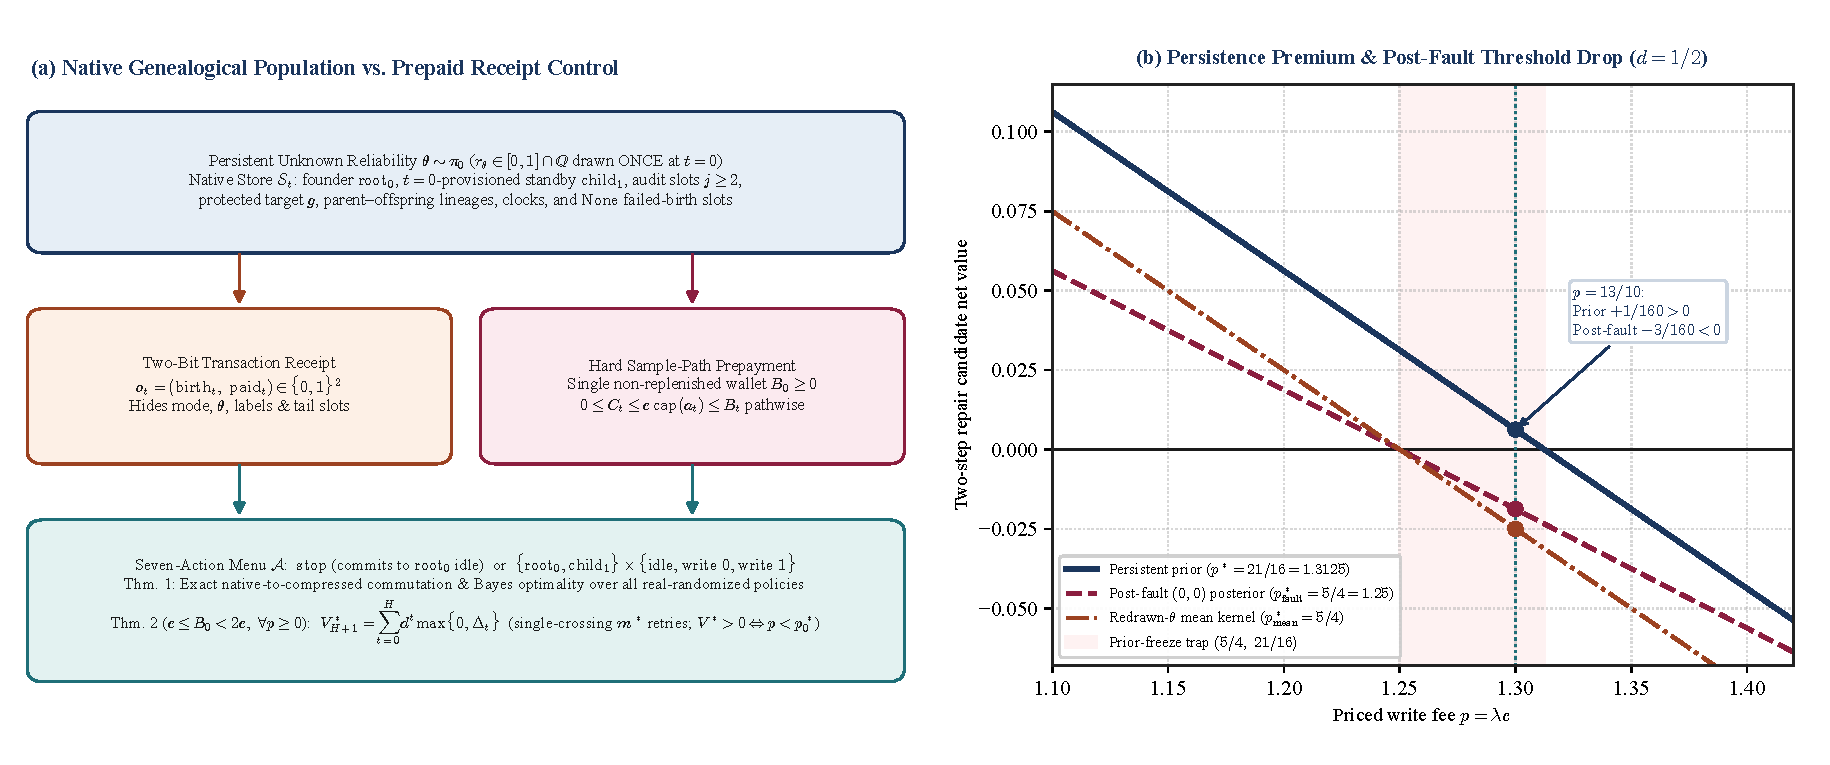
\includegraphics[width=0.99\linewidth,height=\textheight,keepaspectratio,alt={Native
genealogical population protocol and exact two-step repair-threshold
geometry. (a) Separation between the unbounded native genealogical store
\textbackslash mathcal\{S\}\_t (where only t=0 provisions standby
child1) and the controller's two-bit receipt interface o\_t =
(\textbackslash mathrm\{birth\}\_t, \textbackslash mathrm\{paid\}\_t)
under hard sample-path prepayment B\_t \textbackslash ge
c\textbackslash,\textbackslash mathrm\{cap\}(a\_t), alongside the
arbitrary-price single-wallet optimal retry formula of Theorem 2. (b)
Exact two-step repair candidate net value as a function of priced write
fee p = \textbackslash lambda c under equal prior weights on
r\_\textbackslash theta \textbackslash in \textbackslash\{1/4,
3/4\textbackslash\} and d = 1/2 (Theorems 2 and 3), showing the
persistence variance premium d\textbackslash,\textbackslash
mathrm\{Var\}(r\_\textbackslash theta) = 1/32 over a step-redrawn mean
kernel and the strict post-fault threshold contraction from 21/16 to 5/4
creating the prior-freeze trap on (5/4,
21/16).}]{figures/fig1_architecture_and_thresholds.pdf}
\caption{Native genealogical population protocol and exact two-step
repair-threshold geometry. (a) Separation between the unbounded native
genealogical store \(\mathcal{S}_t\) (where only \(t=0\) provisions
standby \protect\texttt{child1}) and the controller's two-bit receipt
interface \(o_t = (\mathrm{birth}_t, \mathrm{paid}_t)\) under hard
sample-path prepayment \(B_t \ge c\,\mathrm{cap}(a_t)\), alongside the
arbitrary-price single-wallet optimal retry formula of Theorem 2. (b)
Exact two-step repair candidate net value as a function of priced write
fee \(p = \lambda c\) under equal prior weights on
\(r_\theta \in \{1/4, 3/4\}\) and \(d = 1/2\) (Theorems 2 and 3),
showing the persistence variance premium
\(d\,\mathrm{Var}(r_\theta) = 1/32\) over a step-redrawn mean kernel and
the strict post-fault threshold contraction from \(21/16\) to \(5/4\)
creating the prior-freeze trap on \((5/4, 21/16)\).}
\end{figure}

\section{Persistence variance premium, post-fault posterior contraction,
and value of
information}\label{persistence-variance-premium-post-fault-posterior-contraction-and-value-of-information}

Writing \(\mu_k := \mathbb{E}_{\pi_0}[r_\theta^k]\) for the \(k\)-th
prior moment of the persistent reliability \(r_\theta\), Theorem 2(3)
shows that whenever \(p \ge p_1^*(H)\) (in particular for
\(p \ge S_H(d)\)), optimal single-wallet values at total horizons \(2\),
\(3\), and \(4\) (\(H = 1, 2, 3\)) specialize to the explicit
prior-moment formulas \[\begin{aligned}
V_2^* &= \max\bigl\{0,\ \mu_1(1 - p) + d\,\mu_2\bigr\}, &\quad p &\ge p_1^*(1) = 1, \\
V_3^* &= \max\bigl\{0,\ \mu_1(1 - p) + (d + d^2)\mu_2\bigr\}, &\quad p &\ge p_1^*(2) = 1 + d\,\frac{\mu_2 - \mu_3}{\mu_1 - \mu_2}, \\
V_4^* &= \max\bigl\{0,\ \mu_1(1 - p) + (d + d^2)\mu_2 + d^3(2\mu_3 - \mu_4)\bigr\}, &\quad p &\ge p_1^*(3).
\end{aligned}\] Comparing these exact expressions against restricted
information regimes---stepwise parameter redrawing, frozen priors after
a fault, open-loop continuation without receipt feedback, and omniscient
\(\theta\)-revelation---yields four sharp structural laws of Bayesian
adaptive maintenance
\citep{blackwell1953, howard1966, easleyKiefer1988, aghion1991, ross2011}.
Throughout Table 1 and Theorem 3, we distinguish cleanly between a
\emph{repair candidate's net value} (committing to initial repair) and
the \emph{restricted-menu optimal value} (which takes
\(\max\{0, \cdot\}\) via \texttt{stop}).

\Needspace{14\baselineskip}

{\def\LTcaptype{none} % do not increment counter
\begin{longtable}[]{@{}
  >{\raggedright\arraybackslash}p{(\linewidth - 4\tabcolsep) * \real{0.3333}}
  >{\raggedright\arraybackslash}p{(\linewidth - 4\tabcolsep) * \real{0.3333}}
  >{\raggedright\arraybackslash}p{(\linewidth - 4\tabcolsep) * \real{0.3333}}@{}}
\toprule\noalign{}
\begin{minipage}[b]{\linewidth}\raggedright
Structural Contrast
\end{minipage} & \begin{minipage}[b]{\linewidth}\raggedright
Exact Formula / Threshold Identity
\end{minipage} & \begin{minipage}[b]{\linewidth}\raggedright
Concrete Verified Rational Witness (\(B_0 = c = 1\))
\end{minipage} \\
\midrule\noalign{}
\endhead
\bottomrule\noalign{}
\endlastfoot
Persistent vs.~redrawn \(\theta\) (\(H=2\)) &
\(V_{2,\mathrm{repair}} - V_{2,\mathrm{redraw}} = d(\mu_2 - \mu_1^2) = d\,\mathrm{Var}(r_\theta)\)
& \(r \in \{1/4, 3/4\}\) eq., \(d=1/2, p=13/10\): \(+1/160\)
vs.~\(-1/40\) (redraw opt. \(0\)) \\
Post-fault \((0,0)\) threshold drop &
\(\Delta p^* = d\frac{\mu_1\mu_3 - \mu_2^2}{\mu_1(\mu_1 - \mu_2)} > 0\)
(\(0 < r_0 < r_1 < 1\)) & Threshold drops \(21/16 \to 5/4\); retry cand.
at \(p=13/10\) gives \(-3/160\) \\
Prior-freeze loss (\(H=3, p \in [p_1^*(2), p_0^*(1))\)) &
\(V_3^* - J_3(\pi_{\mathrm{freeze}}) > 0\) for
\(p \in (p_{\mathrm{fault}}^*(1), p_{\mathrm{prior}}^*(1))\) &
\(r \in \{1/4, 3/4\}\) eq., \(d=1/2, p=13/10\):
\(27/320 - 51/640 = 3/640\) \\
Two-body vs.~root-only cand. (\(H=3\)) & Cand. gap
\((d + d^2)\mu_2 - (d\mu_2 + d^2\mu_3) = d^2(\mu_2 - \mu_3)\) &
\(r \in \{1/4, 3/4\}\) eq., \(d=3/4, p=7/4\): \(V_3^* = +9/256\)
vs.~cand. \(-9/512\) (opt. \(0\)) \\
Receipt feedback vs.~open-loop (\(H=4\)) & Raw cont. gap
\(d^3\mathbb{E}[r_\theta^3(1 - r_\theta)]\); net gap equal when
\(V_{4,\mathrm{open,cand}} \ge 0\) & \(r \in \{3/4, 7/8\}\) eq.,
\(d=3/4, p=37/16\): \(V_4^* - V_{4,\mathrm{open}}^* = 20925/524288\) \\
Post-repair \(\theta\)-revelation (\(\mathrm{EVPI}_{\mathrm{post}}\)) &
\(U_2(r_\theta, d, n)\) attained uniformly by \texttt{freeSchedule} &
\(\mathrm{EVPI}_{\mathrm{post}} = 0\) for \emph{every} prior \(\pi_0\)
and remaining horizon \(n \ge 0\) \\
\end{longtable}
}

Table 1. Exact analytical decompositions and rational witnesses
separating parameter persistence, Bayesian fault updating, two-body
dispatch, receipt feedback, and post-repair parameter revelation.

\textbf{Theorem 3 (Persistence premium, post-fault threshold
contraction, feedback gain, and zero post-repair EVPI).} \emph{Under the
model of Theorem 1 with \(c \le B_0 < 2c\):}

\begin{enumerate}
\def\labelenumi{\arabic{enumi}.}
\tightlist
\item
  \textbf{Persistence variance premium.} \emph{At total horizon \(2\),
  replacing persistent \(\theta \sim \pi_0\) by an i.i.d. redraw
  \(\theta_t \sim \pi_0\) at each step replaces
  \(\mu_2 = \mathbb{E}[r_\theta^2]\) by \(\mu_1^2\), reducing the
  initial-repair candidate net value by
  \(d(\mu_2 - \mu_1^2) = d\,\mathrm{Var}(r_\theta) \ge 0\) (strictly
  positive whenever \(d > 0\) and \(\mathrm{Var}(r_\theta) > 0\)). Under
  equal prior weights on \(r \in \{1/4, 3/4\}\) with \(d = 1/2\) and
  \(p = 13/10\), persistent optimal value is \(V_2^* = 1/160 > 0\),
  whereas the redrawn mean-kernel repair candidate value is
  \(-1/40 < 0\) (so a redrawn-kernel controller must \texttt{stop} for
  optimal value \(0\)).}
\item
  \textbf{Strict post-fault repair-threshold contraction.} \emph{Suppose
  \(\mu_1 < 1\). Conditioning on an uncharged initial fault receipt
  \(o_0 = (0,0)\) after \((0, \mathrm{write}_g)\) leaves wallet
  \(B_1 = B_0 \ge c\) unspent and updates the posterior moments to}
  \[\mu'_k := \mathbb{E}\bigl[r_\theta^k \mid o_0 = (0,0)\bigr] = \frac{\mu_k - \mu_{k+1}}{1 - \mu_1}, \qquad k \ge 1.\]
  \emph{For any nondegenerate two-point prior assigning weight
  \(w \in (0,1)\) to \(r_0\) and \(1 - w\) to \(r_1\) with
  \(0 < r_0 < r_1 < 1\),}
  \[\mu_1\mu_3 - \mu_2^2 = w(1 - w) r_0 r_1 (r_0 - r_1)^2 > 0.\]
  \emph{Consequently, for every \(d > 0\), the remaining two-step repair
  positivity threshold strictly drops after a fault:}
  \[p_{\mathrm{fault}}^*(1) := 1 + d\,\frac{\mu'_2}{\mu'_1} = 1 + d\,\frac{\mu_2 - \mu_3}{\mu_1 - \mu_2} < 1 + d\,\frac{\mu_2}{\mu_1} = p_{\mathrm{prior}}^*(1).\]
  \emph{At \(w = 1/2\), \((r_0, r_1) = (1/4, 3/4)\), and \(d = 1/2\),
  the threshold drops from \(21/16\) to \(5/4 = p_1^*(2)\): at
  \(p = 13/10 \in (5/4, 21/16)\) and total horizon \(3\), Theorem 2(2)
  selects \(m^* = 1\) with \(V_3^* = 27/320\) (halting after \((0,0)\)),
  whereas freezing the prior and retrying yields \(51/640\), incurring
  exact loss \(3/640\) (and at \(p = 6/5 < 5/4\), \(m^* = 2\) becomes
  optimal with \(V_3^* = 89/640\)).}
\item
  \textbf{Open-loop sufficiency at \(H=3\) versus strict
  receipt-feedback gain at \(H=4\).} \emph{At total horizon \(3\)
  (\(B_0 = c\), \(p \ge p_1^*(2)\)), the open-loop action sequence
  \([(0, \mathrm{write}_g), (0, \mathrm{idle}), (1, \mathrm{idle})]\)
  already achieves \(\mu_1(1-p) + (d + d^2)\mu_2 = V_3^*\) whenever
  positive (e.g., at \(r \in \{1/4, 3/4\}, d = 3/4, p = 7/4\),
  \(V_3^* = 9/256 > 0\), whereas the root-only repair candidate
  \([(0, \mathrm{write}_g), (0, \mathrm{idle}), (0, \mathrm{idle})]\)
  yields net value \(-9/512 < 0\), forcing a root-only controller with
  \texttt{stop} to earn optimal value \(0\)). At total horizon \(4\), by
  contrast, after initial repair succeeds and exhausts the wallet, the
  maximum continuation value over all predetermined three-step open-loop
  sequences in \(\{(0, \mathrm{idle}), (1, \mathrm{idle})\}^3\) is
  \(r + dr + d^2 r^2\) (attained by alternating
  \((0, \mathrm{idle}), (1, \mathrm{idle}), (0, \mathrm{idle})\)),
  whereas receipt-adaptive switching achieves
  \(U_2(r, d, 3) = r + dr + d^2(2r^2 - r^3)\), yielding the nonnegative
  raw continuation feedback advantage}
  \[\Delta_{\mathrm{raw}}^{(4)} := d^3\,\mathbb{E}_{\pi_0}\!\bigl[r_\theta^3(1 - r_\theta)\bigr] \ge 0,\]
  \emph{which is strictly positive iff \(d > 0\) and
  \(\mathbb{P}_{\pi_0}(0 < r_\theta < 1) > 0\), and equals the global
  optimal value gap \(V_4^* - V_{4,\mathrm{open}}^*\) whenever
  \(p \ge p_1^*(3)\) and the open-loop repair candidate value
  \(V_{4,\mathrm{open,cand}}\) is nonnegative. At equal weights on
  \(r \in \{3/4, 7/8\}\), \(d = 3/4\), and
  \(p = 37/16 \ge 1 + 3/4 + 9/16\), both repair candidates are strictly
  positive
  (\(V_{4,\mathrm{open}}^* = V_{4,\mathrm{open,cand}} = 2325 / 65536 > 0\)
  and \(V_4^* = 39525 / 524288\)), so
  \(V_4^* - V_{4,\mathrm{open}}^* = \Delta_{\mathrm{raw}}^{(4)} = 20925 / 524288\).}
\item
  \textbf{Exact zero post-repair value of \(\theta\)-revelation.}
  \emph{In the exact same post-repair continuation subgame (\(B = 0\),
  two intact units, arbitrary remaining horizon \(n \in \mathbb{N}\)),
  the parameter-blind receipt policy \texttt{freeSchedule} attains the
  \(\theta\)-omniscient continuation optimum \(U_2(r_\theta, d, n)\)
  pointwise for every \(r_\theta \in [0,1]\). Hence the expected value
  of perfect information on \(\theta\) after repair is identically zero
  (\(\mathrm{EVPI}_{\mathrm{post}} = 0\)), and any positively priced
  auxiliary read of \(\theta\) strictly reduces expected net payoff.}
\end{enumerate}

Theorem 3(3)--(4) (proved in Appendix A.3) places \emph{device-state
feedback} and \emph{parameter revelation} side by side inside the
identical post-repair subgame
\citep{striebel1965, kumarVaraiya1986, krishnamurthy2016}. Revealing the
latent reliability parameter \(\theta\) after wallet exhaustion changes
\emph{parameter uncertainty} without altering the dominant dispatch rule
(\texttt{keep\ idling\ root0\ until\ its\ first\ fault,\ then\ switch\ to\ child1}),
yielding \(\mathrm{EVPI}_{\mathrm{post}} = 0\). Observing two-bit birth
receipts, by contrast, resolves \emph{hidden physical-state
uncertainty}---identifying whether \texttt{root0} faulted on step \(1\)
while \texttt{child1} survived step \(2\) (probability
\((1 - r_\theta)r_\theta\))---routing step \(3\) to the surviving unit
for strictly positive value \(d^3\mathbb{E}[r_\theta^3(1 - r_\theta)]\)
(\(20925 / 524288\) at \(H = 4\)). Notice also that optimizing net
discounted payoff \(J_H\) is distinct from maximizing event
probabilities: in the \(H=2\) and \(H=3\) positive witnesses above,
\(\mathbb{P}(\sum_t \mathrm{birth}_t \ge 1) = 1/2\), and in the \(H=4\)
witness it is \(13/16\).

\section{Informative zero receipts, counting posteriors, and joint
all-action
sufficiency}\label{informative-zero-receipts-counting-posteriors-and-joint-all-action-sufficiency}

\subsection{Separating informative fault observations from deterministic
zero
receipts}\label{separating-informative-fault-observations-from-deterministic-zero-receipts}

When \(B_0 \ge 2c\), multiple paid repairs and post-standby restorations
interact across both slots, so single-wallet closed-form formulas no
longer suffice and exact dynamic programming is required. Over the
general belief space \(\Delta_{\mathbb{Q}}(\mathcal{W}(\Theta))\),
tracking finitely supported world beliefs across quaternary receipts and
seven actions spans \((|\mathcal{A}||\mathcal{O}|)^H = 28^H\) syntactic
action--receipt strings
\citep{papadimitriouTsitsiklis1987, cassandra1997, hauskrecht2000}.
While Bayes-adaptive POMDP models routinely express unknown transition
posteriors through Dirichlet or count statistics
\citep{martin1967, duff2002, ross2011}, compressing our prepaid receipt
process \emph{without approximation loss}
\citep{liWalshLittman2006, subramanian2022} requires solving a sharp
protocol-specific filtering problem: what \emph{finite-coordinate
sufficient operational summary} computed purely from public actions and
two-bit receipts \((a_t, o_t)\) reconstructs the controllable local slot
status, filters out actions whose zero receipts carry zero statistical
information, and preserves exact joint transitions across \emph{all}
legal actions and real-randomized policies?

First, define the finite 24-element \emph{local observer state}
\(q = (x_0, x_1, \mathrm{stopped}, \mathrm{fresh}) \in Q := \{0,1\} \times \{\mathrm{None}, 0, 1\} \times \{0,1\} \times \{0,1\}\)
(\(|Q| = 2 \times 3 \times 2 \times 2 = 24\)), initialized at
\(q_{\mathrm{init}}(g) := (\neg g, \mathrm{None}, 0, 1)\). Here
\(x_0 \in \{0,1\}\) tracks the physical bit of \texttt{root0},
\(x_1 \in \{\mathrm{None}, 0, 1\}\) tracks whether slot \texttt{child1}
is permanently \texttt{None} or holds a unit with bit \(0\) or \(1\),
\(\mathrm{stopped} \in \{0,1\}\) tracks the permanent stop latch, and
\(\mathrm{fresh} \in \{0,1\}\) holds only at \(t = 0\) prior to the
first append (making \(\mathrm{upd}\) a time-homogeneous finite
automaton on \(Q\) without inspecting \(t\); along every reachable
trajectory, \(\mathrm{fresh} = \mathbf{1}_{\{t=0\}}\), restricting \(q\)
to \(12\) local states once \(t \ge 1\)). From \((g, q, a, o)\)
alone---without inspecting the hidden world---the observer updates
\(q' = \mathrm{upd}(g, q, a, o)\) deterministically: writing
\((j_{\mathrm{eff}}, \alpha_{\mathrm{eff}}) = \mathrm{eff}(q.\mathrm{stopped}, a)\)
and \(\beta(g, \mathrm{birth}) := g\) if \(\mathrm{birth} = 1\) else
\(\neg g\), \[\begin{aligned}
x'_0 &:= \begin{cases} x_0, & j_{\mathrm{eff}} = 1, \\ \beta(g, o_1), & j_{\mathrm{eff}} = 0, \end{cases}
&
x'_1 &:= \begin{cases} g, & q.\mathrm{fresh} = 1 \land o_1 = 1, \\ \mathrm{None}, & q.\mathrm{fresh} = 1 \land o_1 = 0, \\ \mathrm{Option.map}(\lambda\_.\,\beta(g, o_1), x_1), & q.\mathrm{fresh} = 0 \land j_{\mathrm{eff}} = 1, \\ x_1, & q.\mathrm{fresh} = 0 \land j_{\mathrm{eff}} = 0, \end{cases}
\end{aligned}\] with
\(\mathrm{stopped}' := q.\mathrm{stopped} \lor \mathbf{1}_{\{a = \mathrm{stop}\}}\)
and \(\mathrm{fresh}' := 0\).

Second, given \((g, q, a)\), let
\(o_{\mathrm{norm}}(g, q, a) \in \{0,1\}^2\) denote the deterministic
receipt that would occur under normal mode \(m = 1\): if the selected
slot in \(q\) is \texttt{None}, \(o_{\mathrm{norm}} = (0,0)\); if the
selected slot holds bit \(x\),
\(o_{\mathrm{norm}} = (\mathbf{1}_{\{x_{\mathrm{cand}}(x, \alpha_{\mathrm{eff}}) = g\}},\, \mathbf{1}_{\{\alpha_{\mathrm{eff}} \neq \mathrm{idle}\}})\).
Under fault mode \(m = 0\), the receipt is \emph{always} \((0,0)\).
Summing out the fair hidden label \(\ell \in \{0,1\}\) gives the exact
single-step marginal receipt likelihood at reliability \(r \in [0,1]\):
\[L_r(o \mid g, q, a) := r\,\mathbf{1}_{\{o = o_{\mathrm{norm}}(g, q, a)\}} + (1 - r)\,\mathbf{1}_{\{o = (0,0)\}}.\]
Observe the critical dichotomy revealed by Table 2: whenever
\(o_{\mathrm{norm}}(g, q, a) = (0,0)\)---which occurs precisely when
idling a damaged slot (\(x = \neg g\)) or dispatching an absent
\texttt{child1} (\(x_1 = \mathrm{None}\))---\emph{both} normal and fault
modes emit \((0,0)\), so \(L_r((0,0) \mid g, q, a) = r + (1 - r) = 1\)
for \emph{every} \(r \in [0,1]\).

\Needspace{14\baselineskip}

{\def\LTcaptype{none} % do not increment counter
\begin{longtable}[]{@{}
  >{\raggedright\arraybackslash}p{(\linewidth - 8\tabcolsep) * \real{0.1818}}
  >{\raggedright\arraybackslash}p{(\linewidth - 8\tabcolsep) * \real{0.1818}}
  >{\centering\arraybackslash}p{(\linewidth - 8\tabcolsep) * \real{0.2273}}
  >{\centering\arraybackslash}p{(\linewidth - 8\tabcolsep) * \real{0.2273}}
  >{\raggedright\arraybackslash}p{(\linewidth - 8\tabcolsep) * \real{0.1818}}@{}}
\toprule\noalign{}
\begin{minipage}[b]{\linewidth}\raggedright
Selected Slot State in \(q\)
\end{minipage} & \begin{minipage}[b]{\linewidth}\raggedright
Effective Action \(\alpha_{\mathrm{eff}}\)
\end{minipage} & \begin{minipage}[b]{\linewidth}\centering
Normal Receipt \(o_{\mathrm{norm}}\)
\end{minipage} & \begin{minipage}[b]{\linewidth}\centering
Fault Receipt
\end{minipage} & \begin{minipage}[b]{\linewidth}\raggedright
Informative? (\(\Delta s + \Delta f = 1\))
\end{minipage} \\
\midrule\noalign{}
\endhead
\bottomrule\noalign{}
\endlastfoot
Existing slot (\(x \in \{0,1\}\)) & \(\mathrm{write}_g\) & \((1, 1)\) &
\((0, 0)\) & \textbf{Yes}: \((1,1) \Rightarrow \Delta s=1\);
\((0,0) \Rightarrow \Delta f=1\) \\
Existing slot (\(x \in \{0,1\}\)) & \(\mathrm{write}_{\neg g}\) &
\((0, 1)\) & \((0, 0)\) & \textbf{Yes}: \((0,1)\) (charged)
\(\Rightarrow \Delta s=1\); \((0,0) \Rightarrow \Delta f=1\) \\
Healthy slot (\(x = g\)) & \(\mathrm{idle}\) & \((1, 0)\) & \((0, 0)\) &
\textbf{Yes}: \((1,0) \Rightarrow \Delta s=1\);
\((0,0) \Rightarrow \Delta f=1\) \\
Damaged slot (\(x = \neg g\)) & \(\mathrm{idle}\) & \((0, 0)\) &
\((0, 0)\) & \textbf{No}: \(L_r((0,0)) \equiv 1\)
(\(\Delta s = \Delta f = 0\)) \\
Absent slot (\(x_1 = \mathrm{None}\)) & Any \(\alpha_{\mathrm{eff}}\) &
\((0, 0)\) & \((0, 0)\) & \textbf{No}: \(L_r((0,0)) \equiv 1\)
(\(\Delta s = \Delta f = 0\)) \\
\end{longtable}
}

Table 2. Exact five-case classification of normal versus fault receipts
(\texttt{RegisterDecisionObserver}), showing why damaged-slot idles and
absent-slot requests produce uninformative zero receipts that must not
increment the fault counter \(f\).

Define the Boolean predicate
\(\mathrm{informative}(g, q, a) :\iff o_{\mathrm{norm}}(g, q, a) \neq (0,0)\)
(equivalently, \(o_{\mathrm{norm},1} \lor o_{\mathrm{norm},2} = 1\)),
and define the step increments
\[\Delta s(g, q, a, o) := \mathbf{1}_{\{\mathrm{informative}(g,q,a) \land o \neq (0,0)\}}, \qquad
\Delta f(g, q, a, o) := \mathbf{1}_{\{\mathrm{informative}(g,q,a) \land o = (0,0)\}}.\]
Calling \(o\) \emph{compatible} with \((g, q, a)\) if
\(o \in \{o_{\mathrm{norm}}(g, q, a),\, (0,0)\}\), the marginal
likelihood factors identically for \emph{all} \(r \in [0,1]\) (retaining
the convention \(0^0 := 1\) at endpoint rates \(r \in \{0,1\}\)) as
\[L_r(o \mid g, q, a) = \mathbf{1}_{\{\mathrm{compatible}(g, q, a, o)\}}\, r^{\Delta s(g, q, a, o)} (1 - r)^{\Delta f(g, q, a, o)}.\]
Folding \((a_t, o_t)\) chronologically along any history
\(h \in (\mathcal{A} \times \mathcal{O})^*\) from
\((0, 0, 0, 0, q_{\mathrm{init}}(g))\) produces the five-coordinate
operational summary
\[\sigma(h) := \bigl(t(h),\ q(h),\ s(h),\ f(h),\ k(h)\bigr) \in \mathbb{N} \times Q \times \mathbb{N} \times \mathbb{N} \times \mathbb{N},\]
where \(t(h) = |h|\) is elapsed time, \(s(h)\) and \(f(h)\) are
cumulative informative normal and fault counts, and
\(k(h) := \sum_{u < |h|} \mathbf{1}_{\{o_{u,2} = 1\}}\) is cumulative
paid writes. Setting
\(w_\theta(s, f) := \pi_0(\theta)\, r_\theta^s (1 - r_\theta)^f\) and
\(Z(s, f) := \sum_{\theta \in \Theta} w_\theta(s, f)\), we obtain
universal posterior sufficiency across \emph{all} real-randomized
policies \citep{halmosSavage1949, dynkin1978}.

\textbf{Theorem 4 (Universal counting-posterior factorization under
arbitrary real-randomized policies).} \emph{Let \(\pi\) be any causal
real-randomized full-history strategy (not assumed to factor through
\(\sigma\), and with arbitrary initial private memory independent of
\(\theta\) and \(\mathcal{S}_0\)). For every history
\(h = [(a_0, o_0), \dots, (a_{t-1}, o_{t-1})] \in (\mathcal{A} \times \mathcal{O})^t\):}

\begin{enumerate}
\def\labelenumi{\arabic{enumi}.}
\tightlist
\item
  \textbf{Likelihood factorization.} \emph{There exists a
  \(\theta\)-independent action-randomization factor
  \(\alpha_\pi(h) \in \mathbb{R}_{\ge 0}\) (the product of \(\pi\)'s
  conditional action probabilities along \(h\)) such that for every
  \(\theta \in \Theta\), the exact native joint probability of
  \((\theta, h)\) is}
  \[\mathbb{P}_{\pi_0, \pi}(\theta, h) = \alpha_\pi(h)\,\mathbf{1}_{\{\mathrm{compat}(h)\}}\, \pi_0(\theta)\, r_\theta^{s(h)} (1 - r_\theta)^{f(h)},\]
  \emph{where \(\mathrm{compat}(h)\) holds iff every step \((a_u, o_u)\)
  in \(h\) is compatible with \((g, q_u, a_u)\). This holds
  unconditionally for all \(\pi_0(\theta) \ge 0\) and all endpoint rates
  \(r_\theta \in [0,1]\) (with \(0^0 = 1\)).}
\item
  \textbf{Exact cancellation on positive-mass histories.} \emph{Whenever
  \(\mathbb{P}_{\pi_0, \pi}(h) = \sum_\theta \mathbb{P}_{\pi_0, \pi}(\theta, h) > 0\),
  necessarily \(\mathrm{compat}(h)\) holds, \(\alpha_\pi(h) > 0\), and
  \(Z(s(h), f(h)) > 0\), so \(\alpha_\pi(h)\) cancels identically and
  the exact conditional posterior is}
  \[\mathbb{P}_{\pi_0, \pi}(\theta \mid h) = \frac{\pi_0(\theta)\, r_\theta^{s(h)} (1 - r_\theta)^{f(h)}}{Z\bigl(s(h), f(h)\bigr)} \in \mathbb{Q} \qquad (\forall \theta \in \Theta).\]
\end{enumerate}

\subsection{Joint all-action sufficiency and necessary versus removable
history
distinctions}\label{joint-all-action-sufficiency-and-necessary-versus-removable-history-distinctions}

Combining local-observer reconstruction with Theorem 4 shows that
\(\sigma = (t, q, s, f, k)\) is a \emph{jointly sufficient decision
state} across the entire action menu
\citep{striebel1965, burkeRosenblatt1958, kemenySnell1960, givanDeanGreig2003},
while reachable three-step trajectories prove that neither \((s,f)\) nor
\(q\) can be dropped and that sufficiency is strictly indexed to the
permitted action menu (Figure 2).

\textbf{Theorem 5 (Joint all-action sufficiency of
\(\sigma = (t, q, s, f, k)\) and three-way sharpness separations).}
\emph{Under the hypotheses of Theorem 1:}

\begin{enumerate}
\def\labelenumi{\arabic{enumi}.}
\tightlist
\item
  \textbf{Joint single-step and multi-step Bellman sufficiency.}
  \emph{If two positive-mass permitted histories \(h_1, h_2\) at
  remaining horizon \(n = H - t\) satisfy
  \(\sigma(h_1) = \sigma(h_2) = (t, q, s, f, k)\), then their literal
  remaining balances coincide (\(B(h_1) = B(h_2) = B_0 - kc \ge 0\)),
  their feasible menus \(\mathrm{menu}(c, B)\) coincide, and for every
  action \(a \in \mathrm{menu}(c, B)\), their one-step joint
  distributions over
  \((o_t,\, \sigma(h_i \mathbin{+\!+} [(a, o_t)]),\, \mathrm{birth}_t,\, C_t,\, B_{t+1})\)
  are identical. By backward induction (\texttt{StepRefinement}), the
  summary dynamic program over \((n, \sigma)\) has the exact same
  optimal value \(V_H^*(b_0, B_0)\) as the full world-belief dynamic
  program over all supported-admissible real-randomized full-history
  policies.}
\item
  \textbf{Insufficiency of the physical Markov state \((t, q, B)\).}
  \emph{Under equal prior weights on \(r \in \{1/4, 3/4\}\) and
  \(B_0 = c = 1\), execute the fixed three-step sequence
  \([(0, \mathrm{write}_g), (0, \mathrm{idle}), (0, \mathrm{idle})]\).
  Reachable histories} \[\begin{aligned}
  h_A &:= \bigl[((0,\mathrm{write}_g),(1,1)),\ ((0,\mathrm{idle}),(1,0)),\ ((0,\mathrm{idle}),(0,0))\bigr], \\
  h_B &:= \bigl[((0,\mathrm{write}_g),(1,1)),\ ((0,\mathrm{idle}),(0,0)),\ ((0,\mathrm{idle}),(0,0))\bigr]
  \end{aligned}\] \emph{have strictly positive prior probabilities
  \(3/32\) and \(3/16\), and reach the identical elapsed time \(t = 3\),
  exhausted wallet \(B_3 = 0\), and local body state
  \(q_* = (\neg g, g, 0, 0)\) (representing slot \(1\) occupied by bit
  \(g\)). Yet because \(h_B\)'s third step idles an already-damaged
  \texttt{root0} (\(\Delta f = 0\)), \(\sigma(h_A)\) has
  \((s,f) = (2,1)\) (\(\pi_{h_A}(1/4) = 1/4\)) whereas \(\sigma(h_B)\)
  has \((s,f) = (1,1)\) (\(\pi_{h_B}(1/4) = 1/2\)), yielding strictly
  distinct next-step birth probabilities under \((1, \mathrm{idle})\):
  \(\mathbb{P}(\mathrm{birth}_3 = 1 \mid h_A) = 5/8 \neq 1/2 = \mathbb{P}(\mathrm{birth}_3 = 1 \mid h_B)\).}
\item
  \textbf{Genuine genealogy-erasing history merger and menu-relative
  boundary.} \emph{Under the same prior and wallet, reachable three-step
  histories} \[\begin{aligned}
  m_A &:= \bigl[((0,\mathrm{write}_g),(1,1)),\ ((0,\mathrm{idle}),(0,0)),\ ((1,\mathrm{idle}),(1,0))\bigr], \\
  m_B &:= \bigl[((0,\mathrm{write}_g),(1,1)),\ ((1,\mathrm{idle}),(1,0)),\ ((0,\mathrm{idle}),(0,0))\bigr]
  \end{aligned}\] \emph{(each with probability \(3/32\) and posterior
  \(\pi(1/4) = 1/4\)) share the exact complete summary
  \(\sigma(m_A) = \sigma(m_B) = (3, q_*, 2, 1, 1)\) and induce identical
  future joint laws across all seven actions in \(\mathcal{A}\), even
  though their native population stores have distinct slot layouts}
  \[[\mathrm{Some}(\neg g),\, \mathrm{Some}(g),\, \mathrm{None},\, \mathrm{Some}(g)]
  \;\neq\;
  [\mathrm{Some}(\neg g),\, \mathrm{Some}(g),\, \mathrm{Some}(g),\, \mathrm{None}],\]
  \emph{distinct parent--offspring identity records, and distinct
  realized past discounted payoffs (\(1 - p + d^2\) vs.~\(1 - p + d\)).
  However, if the action menu is enlarged with \texttt{(2,\ idle)}
  (dispatching slot \(2\)), future birth probabilities diverge
  immediately to \(0\) after \(m_A\) versus \(r_\theta\) (mean \(5/8\))
  after \(m_B\).}
\end{enumerate}

Theorem 5 establishes \emph{universal prior-independent sufficiency}
rather than claiming that \(\sigma = (t, q, s, f, k)\) is the minimal
state quotient for every specialized prior. For general finite
priors---including asymmetric two-point priors such as
\(r_\theta \in \{3/4, 7/8\}\), where posterior odds scale as
\((7/6)^s (1/2)^f\) so unique prime factorization of \(7\) prevents
distinct \((s,f)\) pairs from colliding---both \(s\) and \(f\) are
non-redundant. By contrast, whenever \(\Theta = \{\theta_0, \theta_1\}\)
has \emph{complementary rates} \(r_1 = 1 - r_0 \in (0,1)\) (such as
\(r_\theta \in \{1/4, 3/4\}\), where
\(\mathbb{P}(r_\theta = 3/4 \mid h)/\mathbb{P}(r_\theta = 1/4 \mid h) = (\pi_0(\theta_1)/\pi_0(\theta_0))\,3^{s - f}\)),
the bivariate count \((s,f)\) collapses without loss to the scalar
net-success count \(\delta := s - f \in \{-t, \dots, t\}\). Section 6.2
quantifies both the universal \((s,f)\) graph and this prior-specialized
\(\delta = s - f\) reduction.

\begin{figure}
\centering
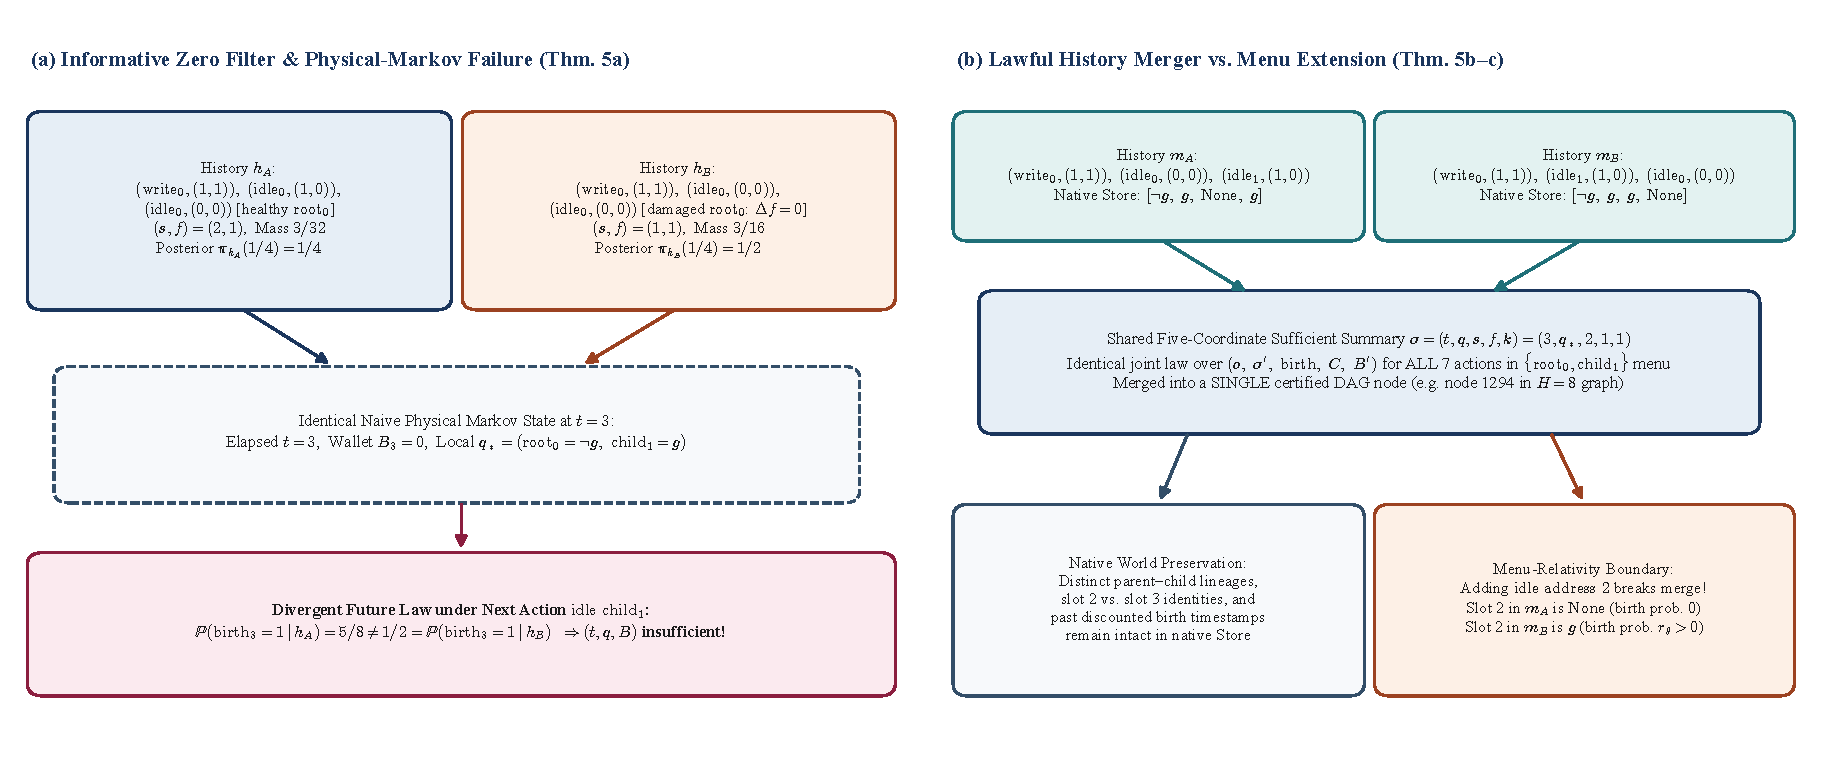
\includegraphics[width=0.99\linewidth,height=\textheight,keepaspectratio,alt={Informative
zero-receipt filtering, physical-Markov failure, and lawful
genealogy-erasing history merger (Theorems 4 and 5). (a) Reachable
histories h\_A and h\_B reach identical elapsed time t=3, wallet B\_3=0,
and local body state q\_* = (\textbackslash neg g, g) yet induce
distinct posteriors and next-step birth probabilities (5/8 vs.~1/2)
because h\_B's third-step zero receipt on a damaged root is
uninformative (\textbackslash Delta f = 0). (b) Reachable histories m\_A
and m\_B with non-isomorphic native genealogical tail stores share exact
five-coordinate summary \textbackslash sigma = (3, q\_*, 2, 1, 1) and
merge into a single certified decision-diagram node under the \{root0,
child1\} menu, while separating (0 vs.~r\_\textbackslash theta) if
slot-2 dispatch is
added.}]{figures/fig2_informative_counts_and_sufficiency.pdf}
\caption{Informative zero-receipt filtering, physical-Markov failure,
and lawful genealogy-erasing history merger (Theorems 4 and 5). (a)
Reachable histories \(h_A\) and \(h_B\) reach identical elapsed time
\(t=3\), wallet \(B_3=0\), and local body state \(q_* = (\neg g, g)\)
yet induce distinct posteriors and next-step birth probabilities
(\(5/8\) vs.~\(1/2\)) because \(h_B\)'s third-step zero receipt on a
damaged root is uninformative (\(\Delta f = 0\)). (b) Reachable
histories \(m_A\) and \(m_B\) with non-isomorphic native genealogical
tail stores share exact five-coordinate summary
\(\sigma = (3, q_*, 2, 1, 1)\) and merge into a single certified
decision-diagram node under the \protect\texttt{\{root0,\ child1\}}
menu, while separating (\(0\) vs.~\(r_\theta\)) if slot-2 dispatch is
added.}
\end{figure}

\section{All-action certifying decision diagrams and polynomial
complexity
bounds}\label{all-action-certifying-decision-diagrams-and-polynomial-complexity-bounds}

\subsection{Separating untrusted memoized graph synthesis from
all-action certificate
checking}\label{separating-untrusted-memoized-graph-synthesis-from-all-action-certificate-checking}

Having shown in Theorem 5 that the five-coordinate summary
\(\sigma = (t, q, s, f, k)\) preserves exact joint single-step
transitions and full-history Bellman values across all legal actions,
how should an implementation construct, store, and \emph{verify} the
resulting shared policy graph? Standard decision-diagram planners in
stochastic control---such as SPUDD and algebraic decision diagrams in
factored MDPs \citep{bryant1986, bahar1997, hoey1999, boutilier2000},
finite-state controller search
\citep{littman1995, hansen1998, meuleau1999, poupartBoutilier2003},
point-based or Monte Carlo POMDP approximations
\citep{pineau2003, spaanVlassis2005, silverVeness2010}, and optimization
decision diagrams \citep{bergman2016}---typically interleave hash-table
memoization, pruning heuristics, and floating-point value updates inside
a single monolithic solver. Proving total correctness of mutable or
hash-indexed graph-building code directly inside a proof assistant can
be brittle and obscures the mathematical structure of the certificate.

Following the \emph{certifying algorithm} paradigm
\citep{blumKannan1995, mcconnell2011}, we separate graph synthesis from
verification across three layered Lean modules: (a) an untrusted
bottom-up generator \texttt{generate} in
\texttt{FiniteJointDecisionDAGGenerator}, (b) a generic all-action
Bellman certificate verifier \texttt{certify} in the module
\texttt{FiniteJointDecisionDAG}, and (c) the source-level acceptance
gate \texttt{accept} in the module
\texttt{RegisterDecisionRepresentation}:

\begin{enumerate}
\def\labelenumi{\arabic{enumi}.}
\tightlist
\item
  \textbf{Untrusted memoized DAG generator (\texttt{generate}).} Given a
  problem instance specified by \((\Theta, \pi_0, r_\cdot, g)\) and
  \((c, B_0, \lambda, d, H)\), \texttt{generate} initializes an empty
  hash map keyed by \((n, \sigma)\)---where \(n = H - t\) is remaining
  horizon---and recursively expands positive-mass receipt successors
  \(m_\sigma^a(o) > 0\) for \emph{every} legal action
  \(a \in \mathrm{menu}(c, \max\{0, B_0 - kc\})\). Completed child nodes
  are appended bottom-up to a flat array
  \(G = [\mathrm{node}_0, \dots, \mathrm{node}_{N_H - 1}]\), so every
  parent edge stores only a bounded integer cursor
  \texttt{idx\ \textless{}\ G.size}. Whenever two distinct histories
  reach the same key \((n, \sigma)\), they reuse the identical array
  index without re-solving the subproblem or materializing the \(28^H\)
  tree.
\item
  \textbf{Two-layer executable acceptance verifier
  (\texttt{accept\ :\ Option\ Result}).} Rather than trusting
  \texttt{generate}, \texttt{accept} inspects a candidate
  \texttt{(G,\ root\_id)} in two explicit stages:

  \begin{itemize}
  \tightlist
  \item
    \emph{Stage A --- Generic all-action Bellman certification
    (\texttt{certify\ :\ Option\ Certified}):} The Boolean verifier
    \texttt{check} checks that every row in \(G\) has a distinct key
    \((n_i, \sigma_i)\), that \texttt{root\_id\ \textless{}\ G.size}
    binds to \((H, \sigma_{\mathrm{init}})\) where
    \(\sigma_{\mathrm{init}} = (0, q_{\mathrm{init}}(g), 0, 0, 0)\),
    that every terminal row (\(n_i = 0\)) stores exact rational value
    \(v_i = 0\), and that every non-terminal row (\(n_i > 0\)) satisfies
    \texttt{NodeValid}: \texttt{check} enumerates \emph{all} legal
    actions \(a \in \mathrm{menu}(c, B(\sigma_i))\)---not merely the
    selected action \(a_i^*\)---verifies that \emph{every} receipt
    \(o \in \mathcal{O}\) with \(m_{\sigma_i}^a(o) > 0\) points to a
    valid index \(j < G.\mathrm{size}\) with key
    \((n_i - 1, \mathrm{updStat}(g, \sigma_i, a, o))\), recomputes
    \[Q_G(i, a) := \sum_{o : m_{\sigma_i}^a(o) > 0} m_{\sigma_i}^a(o)\Bigl[\bigl(\mathbf{1}_{\{o_1 = 1\}} - \lambda c \mathbf{1}_{\{o_2 = 1\}}\bigr) + d\, v_{\mathrm{target}(i, a, o)}\Bigr] \in \mathbb{Q},\]
    and checks
    \(v_i = \max_{a \in \mathrm{menu}(c, B(\sigma_i))} Q_G(i, a)\) with
    canonical tie-breaking in \(\mathcal{A}\).
  \item
    \emph{Stage B --- Source-specific count and time invariant check
    (\texttt{boundCheck}):} Given \texttt{control} returned by
    \texttt{certify}, \texttt{accept} additionally verifies
    \texttt{boundCheck(H,\ G)\ =\ true}---enforcing \(n_i + t_i = H\),
    \(s_i \le t_i\), \(f_i \le t_i\) (with reachable rows satisfying
    \(s_i + f_i \le t_i\)), and \(k_i \le t_i\) on \emph{every} stored
    row of \(G\)---returning \texttt{some\ ⟨control,\ hb⟩}
    (\texttt{Option\ Result}) only when both stages pass
    (\texttt{returned\ :=\ accept(generate(...))}).
  \end{itemize}
\end{enumerate}

Both verification stages are provably non-redundant (and both negative
boundary probes are checked in \texttt{validate.py}). First, why must
\texttt{NodeValid} inside \texttt{certify} check unselected suboptimal
actions? Because storing only the chosen action \(a_i^*\) verifies
\(J_H(G) = v_{\mathrm{root}}\) \emph{without certifying that no
alternative action beats \(a_i^*\)}; deleting a single positive-mass
edge of an unselected action (\texttt{stop}) causes \texttt{certify} to
reject immediately. Second, why is \texttt{boundCheck} inside
\texttt{accept} required for the \(24(H+1)^4\) array size bound? Generic
\texttt{certify} ensures value optimality from \texttt{root\_id},
\emph{not} reachability of auxiliary rows: at \(H = 0\), appending
\(24\) unreachable terminal rows
\((0, (t_i, q_{\mathrm{init}}, 0, 0, 0))\) (\(t_i = 1, \dots, 24\)) with
\(v_i = 0\) behind the valid root yields a \(25\)-row array accepted by
\texttt{certify} yet exceeding \(24(0+1)^4 = 24\), whereas
\texttt{boundCheck} rejects every row violating \(n_i + t_i = H\).

\subsection{Reachable cubic bounds, quartic acceptance ceilings,
rational bit-lengths, and
benchmarks}\label{reachable-cubic-bounds-quartic-acceptance-ceilings-rational-bit-lengths-and-benchmarks}

Once \texttt{accept} returns \texttt{some\ res} for
\((G, \mathrm{root\_id})\), runtime execution (\texttt{packedRun} /
\texttt{nativeRun}) never unfolds \texttt{G} back into a tree: at each
tick \(t\), the controller maintains only an integer node cursor
\(i_t \in \{0, \dots, N_H - 1\}\), issues the stored action
\(a_{i_t}^* \in \mathcal{A}\) to the native genealogical store
\(\mathcal{S}_t\), receives
\(o_t = (\mathrm{birth}_t, \mathrm{paid}_t)\), advances \(i_{t+1}\)
along the certified edge for \((a_{i_t}^*, o_t)\), and falls back to an
explicit safe zero-fee action (\texttt{stop}) on any impossible
zero-mass branch (Figure 3).

\textbf{Theorem 6 (Acceptance soundness, quartic verifier ceiling, cubic
fixed-wallet reachability, and polynomial bit-complexity).}
\emph{Consider any valid rational problem instance over horizon
\(H \in \mathbb{N}\) with write capacity
\(M := \lfloor B_0 / c \rfloor \in \mathbb{N}\).}

\begin{enumerate}
\def\labelenumi{\arabic{enumi}.}
\tightlist
\item
  \textbf{Exact native attainment and full-history real-randomized
  optimality.} \emph{Whenever \texttt{accept} returns \texttt{some\ res}
  on candidate \((G, i_{\mathrm{root}})\) with root value
  \(v_{\mathrm{root}} \in \mathbb{Q}\) (indeed, already whenever
  \texttt{certify} succeeds), executing \(G\) from \(i_{\mathrm{root}}\)
  directly against \(\mathcal{S}_0\) achieves
  \(J_H^{\mathrm{native}}(G) = v_{\mathrm{root}} = V_H^*(b_0, B_0) \ge J_H^{\mathrm{native}}(\pi)\)
  across all supported-admissible real-randomized full-history policies
  \(\pi\), while preserving \(L_H = 1 + H\) native slots, lineages, and
  clocks.}
\item
  \textbf{Unconditional sample-path prepayment safety.} \emph{For every
  \texttt{accept}-verified (or \texttt{certify}-verified) array \(G\),
  menu-feasibility of every stored node action guarantees that on every
  positive-prior \(\theta\) and positive-weight primitive noise tape
  \((z_0, \dots, z_{H-1})\), every prefix \(m \le H\) satisfies
  pre-execution affordability \(c\,\mathrm{cap}(a_t) \le B_t\)
  (\(t < m\)) and literal balance conservation}
  \[B_m = B_0 - \sum_{t=0}^{m-1} C_t \ge 0, \qquad 0 \le \sum_{t=0}^{m-1} C_t \le B_0.\]
\item
  \textbf{Explicit quartic \texttt{accept}-array ceiling.} \emph{Every
  candidate accepted by \texttt{accept} (\texttt{certify} together with
  \texttt{boundCheck}, counting all stored rows even if unreachable)
  satisfies} \[N_H := G.\mathrm{size} \le 24\,(H + 1)^4.\]
\item
  \textbf{Canonical generator completeness, fixed-wallet cubic reachable
  size, and polynomial rational bit-length.} \emph{For every valid
  rational instance, bottom-up memoized synthesis (\texttt{generate})
  terminates, produces a duplicate-free reachable array
  \(G_{\mathrm{reach}}\) passing \textbf{both} \texttt{certify} and
  \texttt{boundCheck}
  (\texttt{accept(G\_\{\textbackslash{}mathrm\{reach\}\})\ =\ some\ res},
  so \texttt{returned} succeeds), and satisfies the reachable node and
  positive-edge bounds}
  \[|G_{\mathrm{reach}}| \le N_{\mathrm{reach}}(H, M) := 1 + 12 \sum_{t=1}^{H} \binom{t+2}{2}\bigl(\min(M, t) + 1\bigr) = O\Bigl(1 + \bigl(\min(M, H) + 1\bigr)H^3\Bigr),\]
  \emph{with at most \(14\,|G_{\mathrm{reach}}|\) positive-mass edges
  (and under complementary two-point priors \(r_1 = 1 - r_0\) using
  \(\delta = s - f\), at most
  \(1 + 12\sum_{t=1}^H (2t + 1)(\min(M, t) + 1) = O(1 + (\min(M, H) + 1)H^2)\)
  nodes). Moreover, if \(D_0, D_r, D_d, D_p \in \mathbb{N}_{\ge 1}\) are
  common denominators for \(\pi_0\), \(\{r_\theta\}\), \(d\), and
  \(\lambda c\), telescoping cancellation
  \(Z(s,f)\,m_\sigma^a(o) = Z(s + \Delta s, f + \Delta f)\) ensures
  \(D_0 D_r^H D_p D_d^{H-t} Z(s,f)\,V_{H-t}^{\mathrm{stat}}(\sigma) \in \mathbb{Z}\),
  bounding reduced numerator and denominator bit-lengths of every node
  value and edge probability by}
  \[O\Bigl(1 + \log(D_0 D_p) + \log\bigl(1 + H(1 + \lambda c)\bigr) + H\log(D_r D_d)\Bigr)\]
  \emph{(\(O(H)\) bits for fixed numerical parameters, so synthesis and
  \texttt{accept} verification run in time polynomial in the horizon
  \(H\) for fixed \(|\Theta|\) and fixed parameter bit-lengths).}
\end{enumerate}

Theorem 6 (Parts 1--3 mechanized in Lean 4 via
\texttt{RegisterDecisionRepresentation}; Part 4 proved in Appendix A.6)
separates \emph{verifier-level array bounds} from \emph{reachable
state-space and bit-level complexity}. While \texttt{accept} enforces
\(N_H \le 24(H+1)^4\) over arbitrary candidate arrays, every reachable
node at \(t \ge 1\) has \texttt{fresh} \(= 0\) (\(12\) local states in
\(Q\)), \(s + f \le t\) (\(\binom{t+2}{2}\) count pairs), and
\(k \le \min(M, t)\), giving \(O(1 + H^3)\) nodes for any fixed repair
capacity \(M\) (including \(M = 0\)) and \(O(1 + H^2)\) under
complementary two-point log-odds. Crucially, Table 3 benchmarks
compression against the \emph{exact number of legal positive-probability
full histories} (leaves of the unmerged feasible decision--receipt tree)
alongside standalone \texttt{generate} and \texttt{accept} wall-clock
medians (\texttt{python3\ validate.py\ -\/-benchmark-timings}).

\Needspace{14\baselineskip}

{\def\LTcaptype{none} % do not increment counter
\begin{longtable}[]{@{}
  >{\raggedright\arraybackslash}p{(\linewidth - 10\tabcolsep) * \real{0.1600}}
  >{\centering\arraybackslash}p{(\linewidth - 10\tabcolsep) * \real{0.2000}}
  >{\raggedleft\arraybackslash}p{(\linewidth - 10\tabcolsep) * \real{0.1600}}
  >{\raggedleft\arraybackslash}p{(\linewidth - 10\tabcolsep) * \real{0.1600}}
  >{\raggedleft\arraybackslash}p{(\linewidth - 10\tabcolsep) * \real{0.1600}}
  >{\raggedleft\arraybackslash}p{(\linewidth - 10\tabcolsep) * \real{0.1600}}@{}}
\toprule\noalign{}
\begin{minipage}[b]{\linewidth}\raggedright
Benchmark (\(c = 1, g = 1\)) \& \((H, B_0, d, \lambda)\), Prior
\end{minipage} & \begin{minipage}[b]{\linewidth}\centering
Exact Optimal Value \(V_H^*\)
\end{minipage} & \begin{minipage}[b]{\linewidth}\raggedleft
Cert. / Exec. (Nodes / Edges)
\end{minipage} & \begin{minipage}[b]{\linewidth}\raggedleft
Legal Pos. Histories (vs.~\(28^H\))
\end{minipage} & \begin{minipage}[b]{\linewidth}\raggedleft
\(N_{\mathrm{reach}}\) Bound (vs.~\(24(H\!+\!1)^4\))
\end{minipage} & \begin{minipage}[b]{\linewidth}\raggedleft
Gen.~/ Accept (ms)
\end{minipage} \\
\midrule\noalign{}
\endhead
\bottomrule\noalign{}
\endlastfoot
1. Two-step \((2, 1, \frac{1}{2}, \frac{13}{10})\),
\(\{\frac{1}{4}, \frac{3}{4}\}\) & \(\dfrac{1}{160}\) & \(21/43\)
\(\cdot\) \(6/5\) & \(70\) (\(784\)) & \(217\) (\(1,944\)) &
\(1.1\ /\ 1.0\) \\
2. Backup \((3, 1, \frac{3}{4}, \frac{7}{4})\),
\(\{\frac{1}{4}, \frac{3}{4}\}\) & \(\dfrac{9}{256}\) & \(52/127\)
\(\cdot\) \(11/10\) & \(502\) (\(21,952\)) & \(457\) (\(6,144\)) &
\(3.0\ /\ 3.0\) \\
3. Posterior \((3, 1, \frac{1}{2}, \frac{13}{10})\),
\(\{\frac{1}{4}, \frac{3}{4}\}\) & \(\dfrac{27}{320}\) & \(52/127\)
\(\cdot\) \(11/10\) & \(502\) (\(21,952\)) & \(457\) (\(6,144\)) &
\(3.0\ /\ 3.0\) \\
4. Feedback \((4, 1, \frac{3}{4}, \frac{37}{16})\),
\(\{\frac{3}{4}, \frac{7}{8}\}\) & \(\dfrac{39525}{524288}\) &
\(104/287\) \(\cdot\) \(16/16\) & \(3,466\) (\(6.15\times 10^5\)) &
\(817\) (\(15,000\)) & \(6.8\ /\ 6.7\) \\
5. Two-wallet \((8, 2, \frac{3}{4}, \frac{13}{10})\),
\(\{\frac{1}{4}, \frac{3}{4}\}\) & \(\dfrac{884450457}{1342177280}\) &
\(1,661/8,221\) \(\cdot\) \(151/182\) & \(23,841,395\)
(\(3.78\times 10^{11}\)) & \(5,869\) (\(157,464\)) & \(179\ /\ 179\) \\
\end{longtable}
}

Table 3. Exact rational values, certified all-action and execution DAG
sizes, legal positive-probability history leaf counts, fixed-wallet
cubic reachable bounds (\(N_{\mathrm{reach}}\)) versus quartic
\texttt{accept} ceilings, and standalone \texttt{generate} /
\texttt{accept} median times over \(5\) single-core runs
(\texttt{python3\ validate.py\ -\/-benchmark-timings}, arm64 macOS,
CPython 3.9 \texttt{Fraction}; exact values and counts identically
verified in Lean 4).

Table 3 and Figure 3 display the complete hierarchy across all five
benchmarks, highlighted by the eight-step two-repair problem
(\(H = 8, B_0 = 2, c = 1, d = 3/4, \lambda = 13/10\), equal prior on
\(r_\theta \in \{1/4, 3/4\}\)). Filtering incompatible receipts and
infeasible post-exhaustion writes already trims
\(28^8 = 377,801,998,336\) syntactic strings down to
\textbf{\(23,841,395\) legal positive-probability full histories};
merging equivalent \((n, \sigma)\) histories further compresses this
feasible tree by four orders of magnitude into \textbf{\(1,661\)
certified all-action nodes and \(8,221\) edges} (below the cubic
reachable bound \(N_{\mathrm{reach}}(8, 2) = 5,869\) and quartic ceiling
\(157,464\)), synthesized in \(0.18\text{ s}\) (\texttt{178.9\ ms}
median) and independently verified by \texttt{accept} in
\(0.18\text{ s}\) (\texttt{179.4\ ms} median) with maximum reduced
denominator bit-length \(31\) bits (\(1342177280 = 5 \times 2^{28}\)).
Exploiting the complementary prior symmetry \(r_1 = 1 - r_0\) via
\(\delta = s - f\) compresses the same \(H = 8\) all-action graph
further to \textbf{\(1,020\) nodes and \(5,558\) edges} (\(-38.6\%\)
nodes, \(-32.4\%\) edges) with the identical optimal value
\(884450457 / 1342177280 \approx 0.658967\), while the runtime execution
subgraph visits \textbf{\(151\) nodes and \(182\) edges} (achieving
birth probability \(215 / 256 \approx 0.8398\), double-write probability
\(1233 / 4096 \approx 0.3010\), expected undiscounted births
\(57313 / 16384 \approx 3.4981\), and expected undiscounted fees
\(4673 / 4096 \approx 1.1409\)).

\begin{figure}
\centering
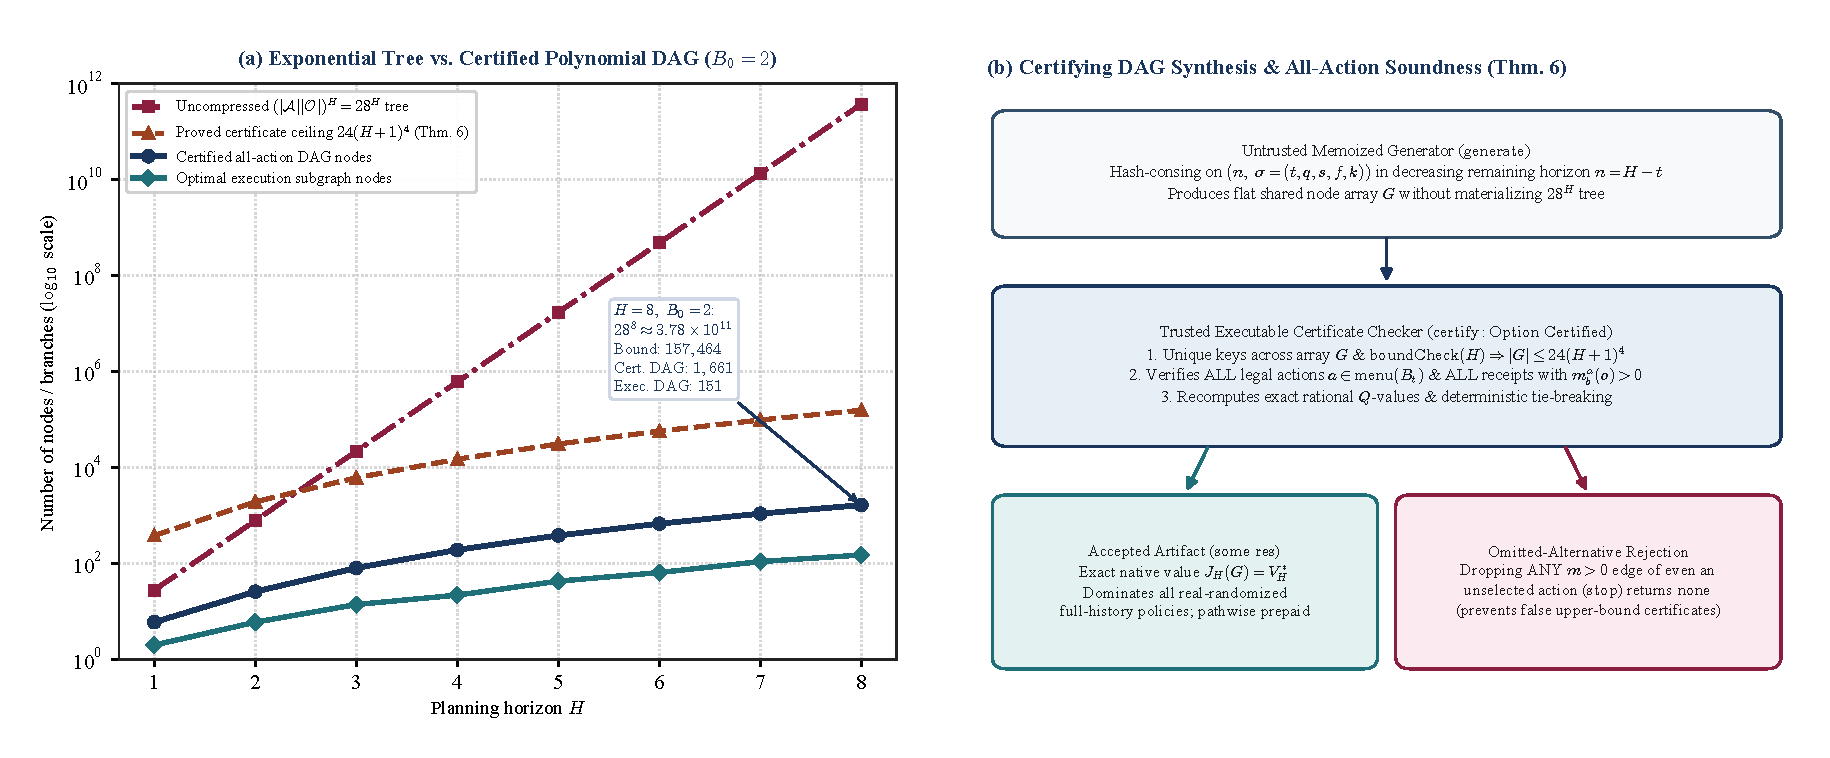
\includegraphics[width=0.99\linewidth,height=\textheight,keepaspectratio,alt={Feasible
history-tree scaling versus polynomial decision-diagram compression and
two-stage certifying architecture (Theorem 6). (a) Logarithmic scaling
across H \textbackslash in \textbackslash\{1, \textbackslash dots,
8\textbackslash\} at B\_0 = 2, c = 1, d = 3/4, \textbackslash lambda =
13/10 (r\_\textbackslash theta \textbackslash in \textbackslash\{1/4,
3/4\textbackslash\} eq.) comparing syntactic 28\^{}H strings, actual
legal positive-probability full histories (23,841,395 at H=8), the
quartic accept ceiling 24(H+1)\^{}4 (157,464), the fixed-wallet cubic
reachable bound N\_\{\textbackslash mathrm\{reach\}\}(H,2) (5,869),
certified (s,f) DAG nodes (1,661), complementary-prior (s-f) DAG nodes
(1,020), and optimal execution nodes (151). (b) Separation between
untrusted memoized DAG synthesis (generate) and the two-layer executable
verifier accept : Option Result (certify + boundCheck), rejecting both
omitted unselected-action branches and out-of-domain
rows.}]{figures/fig3_dag_compression_and_scaling.pdf}
\caption{Feasible history-tree scaling versus polynomial
decision-diagram compression and two-stage certifying architecture
(Theorem 6). (a) Logarithmic scaling across \(H \in \{1, \dots, 8\}\) at
\(B_0 = 2, c = 1, d = 3/4, \lambda = 13/10\)
(\(r_\theta \in \{1/4, 3/4\}\) eq.) comparing syntactic \(28^H\)
strings, actual legal positive-probability full histories
(\(23,841,395\) at \(H=8\)), the quartic \protect\texttt{accept} ceiling
\(24(H+1)^4\) (\(157,464\)), the fixed-wallet cubic reachable bound
\(N_{\mathrm{reach}}(H,2)\) (\(5,869\)), certified \((s,f)\) DAG nodes
(\(1,661\)), complementary-prior \((s-f)\) DAG nodes (\(1,020\)), and
optimal execution nodes (\(151\)). (b) Separation between untrusted
memoized DAG synthesis (\protect\texttt{generate}) and the two-layer
executable verifier \protect\texttt{accept\ :\ Option\ Result}
(\protect\texttt{certify} + \protect\texttt{boundCheck}), rejecting both
omitted unselected-action branches and out-of-domain rows.}
\end{figure}

\section{Formalization architecture, related literature, and explicit
scope
boundaries}\label{formalization-architecture-related-literature-and-explicit-scope-boundaries}

\subsection{Pure-kernel Lean 4 formalization and exact rational
certificate
checking}\label{pure-kernel-lean-4-formalization-and-exact-rational-certificate-checking}

All native and compressed transitions, prepayment invariants, high-price
continuation formulas (\(B_0 = c, p \ge S_H(d)\)), value-of-information
witnesses, counting-posterior factorizations, five-coordinate
sufficiency theorems, and \texttt{accept} (\texttt{certify} +
\texttt{boundCheck}) soundness and quartic size bounds in Sections 2--6
have been formalized in Lean 4 (v4.33.1) over Mathlib
\citep{mouraUllrich2021, mathlib2020} across 30 interconnected modules
(\texttt{FiniteJointDecision*}, \texttt{RegisterJointDecision*}, and
\texttt{RegisterDecision*}), while the arbitrary-price single-repair
stopping extension across \(c \le B_0 < 2c\) (Theorem 2(2)--(3)) and
canonical generator/bit-length bounds (Theorem 6(4)) are proved
self-containedly in Appendix A.2 and A.6 and cross-checked by our
exact-rational validation suite (\texttt{validate.py}). Across the
entire compiled Lean environment, an automated axiom audit confirms zero
occurrences of \texttt{sorryAx} and zero occurrences of compiler-trusted
evaluation (\texttt{Lean.ofReduceBool} / \texttt{native\_decide})
\citep{boespflug2011}, leaving solely Lean's three standard logical
axioms \texttt{\{propext,\ Classical.choice,\ Quot.sound\}}
\citep{carneiro2019}.

Architecturally, the formalization enforces three methodological
safeguards that complement prior mechanized developments in probability,
information theory, and Markov decision processes
\citep{nipkowPaulsonWenzel2002, bertotCasteran2004, affeldt2014, eberl2015, hoelzl2017, vajjha2021, schaeffelerAbdulaziz2023}
as well as probabilistic model checking
\citep{baierKatoen2008, kwiatkowska2011}:

\begin{enumerate}
\def\labelenumi{\arabic{enumi}.}
\tightlist
\item
  \textbf{Non-circular derivation of sufficiency
  (\texttt{initial\_relation} and \texttt{StepRefinement}).} Rather than
  axiomatizing a reduced state space \(\Sigma\) as primitive, our
  formalization constructs---in the modules
  \texttt{RegisterDecisionObserverSource} and
  \texttt{RegisterDecisionRepresentationModel}---an explicit world-level
  simulation relation \texttt{Rel} linking full finitely supported
  beliefs over \(\mathcal{W}(\Theta)\) to \(\sigma = (t, q, s, f, k)\),
  proves \texttt{initial\_relation} on the damaged founder
  \(\mathcal{S}_0\), and discharges \texttt{StepRefinement} for every
  legal action and positive-mass receipt.
\item
  \textbf{Separation between noncomputable real expectations and
  executable rational artifacts.} Native genealogical expectations
  (\texttt{nativeTotal}, \texttt{expectedRawNativeJ}) are formulated
  over \(\mathbb{R}\) and \texttt{PMF} to interface cleanly with general
  real-randomized competitors (\texttt{RawCausalPolicy}), whereas
  \texttt{summarize}, \texttt{countBelief}, \texttt{generate},
  \texttt{certify}, \texttt{boundCheck}, \texttt{accept}, and
  \texttt{packedRun} execute purely over computable Lean types
  (\texttt{Nat}, \texttt{Rat}, \texttt{Bool}, \texttt{Option},
  \texttt{Array}). Exact bridge theorems
  (\texttt{checked\_native\_value}, \texttt{checked\_native\_optimal},
  \texttt{initial\_graph\_native\_payment},
  \texttt{result\_node\_bound}) equate the two layers without runtime
  real arithmetic.
\item
  \textbf{Explicit \texttt{Option} acceptance boundary (\texttt{accept}
  returning \texttt{Option\ Result}).} Following \citep{mcconnell2011},
  \texttt{FiniteJointDecisionDAG} proves Bellman soundness of
  \texttt{certify}, while \texttt{accept} in
  \texttt{RegisterDecisionRepresentation} adds \texttt{boundCheck} to
  guarantee \texttt{result\_node\_bound} (\(N_H \le 24(H+1)^4\)) without
  requiring mutable hash-table invariants inside the trusted kernel.
  Theorem 6(4) proves mathematically that \texttt{generate} always
  passes both \texttt{certify} and \texttt{boundCheck}
  (\texttt{returned} evaluates \texttt{accept} on \texttt{generate} to
  \texttt{some\ res}), and all five main benchmarks (Table 3) plus eight
  boundary stress tests (\(H = 0\), \(B_0 = 0\), \(B_0 < c\), endpoint
  rates \(r \in \{0,1\}\), zero-weight prior atoms, duplicate rate
  atoms, and inverted target \(g = 0\)) are explicitly generated and
  kernel-checked.
\end{enumerate}

\subsection{Comparison with classical operations research and explicit
scope
boundaries}\label{comparison-with-classical-operations-research-and-explicit-scope-boundaries}

Our results bridge several distinct literatures in stochastic control
and operations research:

\begin{itemize}
\tightlist
\item
  \textbf{Partially observed replacement vs.~initialization-epoch
  standby provisioning.} Classical multitype branching optimization
  \citep{harris1963, sevastyanov1971, athreyaNey1972, pliska1976, rothblumWhittle1982, gonzalez2018}
  characterizes asymptotic Perron eigenvalues under full census
  observation, partially observed maintenance
  \citep{eckles1968, ross1971, barlowProschan1975, white1979, monahan1982, makisJiang2003}
  analyzes single-unit deterioration without standby commissioning or
  outcome-contingent billing, and Markovian cold/warm standby
  control-limit models \citep{barronYechiali2017} assume known
  deterioration rates and repeatable repair access. Our model centers on
  the three-way interaction of a \emph{one-time step-\(0\) standby
  provisioning window} (\texttt{child1}), \emph{persistent reliability
  learning} (\(\theta \sim \pi_0\)), and \emph{uncharged-fault
  prepayment retries} (\(B_0 \ge 0\)), yielding complete nested
  retry-stopping thresholds across \(c \le B_0 < 2c\) and exact
  multi-wallet DAG synthesis at \(B_0 \ge 2c\).
\item
  \textbf{Bayesian adaptive control, Bernoulli stopping, and constrained
  MDPs.} In one-armed Bernoulli bandits, geometric-discount optimal
  stopping, and Bayes-adaptive POMDPs
  \citep{robbins1952, bellman1961, rieder1975, gittins1979, berryFristedt1979, whittle1982, fristedtBerry1988, easleyKiefer1988, aghion1991, duff2002, ross2011},
  pulling an uncertain arm yields stationary rewards, while constrained
  MDPs
  \citep{altman1999, feinberg2000, bauerleRieder2011, mannorTsitsiklis2013}
  or knapsack bandits \citep{besbesZeevi2009, badanidiyuru2018} impose
  expected or deterministic budgets. Here, paid intervention ends upon
  the \emph{first} successful repair (\(B_0 - c < c\)), failures are
  uncharged yet shift the posterior downward, and step-\(0\) failure
  closes the standby bay---producing single-crossing retry thresholds
  (\(p_0^* \ge p_1^* \ge \dots \ge p_H^*\)), a persistence variance
  premium (\(d\,\mathrm{Var}(r_\theta)\)), and strictly positive
  post-repair \emph{device-state} feedback
  (\(d^3\mathbb{E}[r_\theta^3(1-r_\theta)]\)) inside the exact subgame
  where \emph{parameter} revelation is worthless
  (\(\mathrm{EVPI}_{\mathrm{post}} = 0\)).
\item
  \textbf{Sufficient statistics and certifying decision diagrams.}
  Whereas general POMDP belief spaces remain continuous
  \citep{smallwoodSondik1973, sondik1978, lovejoy1991, kaelbling1998}---motivating
  approximate information states \citep{subramanian2022} or bounded
  controllers \citep{hansen1998, poupartBoutilier2003}---Theorems 4--6
  identify exact local state reconstruction and uninformative
  zero-receipt filtering on \(\mathcal{A}\), yielding
  \(O(1 + (\min(M, H) + 1)H^3)\) reachable all-action certifying DAGs
  (\(O(1 + (\min(M, H) + 1)H^2)\) under complementary two-point priors)
  with \(O(H)\) reduced rational bit-lengths for fixed numerical
  parameters
  \citep{bryant1986, bahar1997, hoey1999, bergman2016, mcconnell2011}.
\end{itemize}

At the same time, three scope boundaries must be stated explicitly:

\begin{enumerate}
\def\labelenumi{\arabic{enumi}.}
\tightlist
\item
  \emph{Fixed-menu polynomial tractability versus general POMDPs and
  large \(|\Theta|\).} Theorem 6(4) establishes
  \(O(1 + (\min(M, H) + 1)H^3)\) reachable nodes and polynomial-in-\(H\)
  rational synthesis and \texttt{accept} verification for fixed dispatch
  slots \texttt{\{root0,\ child1\}}, fixed finite prior support
  \(\Theta\) (with each node's posterior expectation summing over
  \(|\Theta|\) atoms), and fixed parameter bit-lengths; it does
  \emph{not} claim polynomial-time solvability for general POMDPs
  \citep{papadimitriouTsitsiklis1987, madani2003}, and external solver
  CPU/memory lies outside the physical wallet \(B_0\).
\item
  \emph{Menu-relativity and known-target alignment.} Both compressed
  commutation (Theorem 1) and five-coordinate sufficiency (Theorem 5)
  rely on known public target alignment (\(\mathrm{prog} = g\)) and
  dispatch restricted to addresses \(\{0, 1\}\). As Theorem 5(3)
  demonstrates, granting dispatch access to slot \(2\) immediately
  requires refining \(\sigma\); unknown target programs, simultaneous
  whole-population aging, or correlated whole-store faults constitute
  distinct mathematical problems.
\item
  \emph{Finite-horizon zero-terminal contract versus infinite-horizon
  persistence.} Optimality here holds strictly for the pre-specified
  discounted net output \(J_H\) with zero terminal salvage value and
  zero external income, and should not be conflated with
  infinite-horizon survival or asymptotic lineage growth.
\end{enumerate}

\appendix

\section{Appendix: Self-contained mathematical
proofs}\label{appendix-self-contained-mathematical-proofs}

\subsection{Proof of Theorem 1 (Commutation, prepayment, and
full-history Bayes
optimality)}\label{proof-of-theorem-1-commutation-prepayment-and-full-history-bayes-optimality}

\textbf{(1) Exact native-to-compressed commutation.} Proceed by
induction on \(t \in \{0, \dots, H\}\). At \(t = 0\),
\(\mathcal{S}_0 = [\mathrm{Some}(p_0)]\) has length \(L_0 = 1\),
\(\mathrm{prog}(p_0) = g\) so \(\mathrm{Aligned}(g, \mathcal{S}_0)\)
holds, and
\(\mathrm{project}(\mathcal{S}_0) = [\mathrm{Some}(\neg g)]\). Suppose
at step \(t\) that \(\mathrm{Aligned}(g, \mathcal{S}_t)\) holds,
\(L_t = 1 + t\), and \(s_t = \mathrm{project}(\mathcal{S}_t)\). Let
\((j_{\mathrm{eff}}, \alpha_{\mathrm{eff}}) = \mathrm{eff}(\mathrm{stopped}_t, a_t)\)
and \(z_t = (m_t, \ell_t) \in \{0,1\}^2\).

\begin{itemize}
\tightlist
\item
  \emph{Case 1: \(\mathcal{S}_t[j_{\mathrm{eff}}] = \mathrm{None}\) (or
  \(j_{\mathrm{eff}} \ge L_t\)).} By definition of \texttt{project},
  \(s_t[j_{\mathrm{eff}}] = \mathrm{None}\) as well. Both native and
  compressed transitions leave existing slots \(0, \dots, L_t - 1\)
  unchanged, append \texttt{None} at index \(L_t\) (so
  \(L_{t+1} = L_t + 1 = 1 + (t+1)\) and
  \(\mathrm{Aligned}(g, \mathcal{S}_{t+1})\) is preserved), emit receipt
  \(o_t = (0,0)\), and charge literal fee \(C_t = 0\).
\item
  \emph{Case 2: \(\mathcal{S}_t[j_{\mathrm{eff}}] = \mathrm{Some}(p)\)
  with physical bit \(x \in \{0,1\}\).} Then
  \(s_t[j_{\mathrm{eff}}] = \mathrm{Some}(x)\), and by
  \(\mathrm{Aligned}(g, \mathcal{S}_t)\), \(\mathrm{prog}(p) = g\). In
  the native transaction, the post-step parent organism \(p'\) at slot
  \(j_{\mathrm{eff}}\) retains \(\mathrm{prog}(p') = g\) and updates its
  physical bit to \(x' = x_{\mathrm{cand}}(x, \alpha_{\mathrm{eff}})\)
  if \(m_t = 1\) and \(\neg g\) if \(m_t = 0\), matching
  \(\mathrm{postBit}(g, x, \alpha_{\mathrm{eff}}, m_t)\). Because
  \(\mathrm{prog}(p) = g\), a newborn \(c_{\mathrm{new}}\) is created in
  the native transaction iff \(m_t = 1\) and
  \(x' = \mathrm{prog}(p) = g\), in which case
  \(\mathrm{phys}(c_{\mathrm{new}}) = g\) and
  \(\mathrm{prog}(c_{\mathrm{new}}) = g\), matching
  \(\mathrm{childBit}(g, x, \alpha_{\mathrm{eff}}, m_t) = \mathrm{Some}(g)\)
  and preserving \(\mathrm{Aligned}(g, \mathcal{S}_{t+1})\); otherwise
  \texttt{None} is appended in both stores. Thus
  \(\mathrm{project}(\mathcal{S}_{t+1}) = s_{t+1}\),
  \(L_{t+1} = L_t + 1\), and both receipt bits
  \((\mathrm{birth}_t, \mathrm{paid}_t) = (\mathbf{1}_{\{\mathrm{childBit} \neq \mathrm{None}\}},\, \mathbf{1}_{\{m_t = 1 \land \alpha_{\mathrm{eff}} \neq \mathrm{idle}\}})\)
  and literal fee \(C_t = c\,\mathrm{paid}_t\) agree identically.
\end{itemize}

\textbf{(2) Strict sample-path prepayment.} For every world \(w\),
action \(a \in \mathcal{A}\), and noise \(z = (m, \ell)\), inspect
\(\mathrm{paid}(w, a, z) \in \{0,1\}\)
vs.~\(\mathrm{cap}(a) \in \{0,1\}\): if
\(a \in \{\mathrm{stop}, (0,\mathrm{idle}), (1,\mathrm{idle})\}\), then
\(\alpha_{\mathrm{eff}} = \mathrm{idle}\), so
\(\mathrm{paid}(w,a,z) = 0 = \mathrm{cap}(a)\); if
\(a = (j, \mathrm{write}_v)\), then
\(\mathrm{cap}(a) = 1 \ge \mathrm{paid}(w,a,z)\) regardless of whether
\(w.\mathrm{stopped} = 1\), \(s[j] = \mathrm{None}\), or \(m = 0\).
Hence \(0 \le C_t = c\,\mathrm{paid}_t \le c\,\mathrm{cap}(a_t)\) holds
pathwise. On any prefix \(h_t\) of strictly positive probability under a
supported-admissible policy \(\pi\), every prefix \(h_s\) (\(s < t\))
also has strictly positive probability and \(\pi_s(h_s)(a_s) > 0\), so
\(a_s \in \mathrm{menu}(c, B_s)\), meaning
\(c\,\mathrm{cap}(a_s) \le B_s\). By induction on \(s = 0, \dots, t\):
\(B_0 \ge 0\), and if \(B_s = B_0 - \sum_{u < s} C_u \ge 0\), then
\(B_s - C_s \ge B_s - c\,\mathrm{cap}(a_s) \ge 0\), so
\(\max\{0, B_s - C_s\} = B_s - C_s = B_0 - \sum_{u \le s} C_u \ge 0\).

\textbf{(3) Attainment and optimality over real-randomized full-history
policies.} By Part (1), for every fixed \((\theta, z_{0:H-1})\) and
action sequence \(a_{0:H-1}\), native discounted net payoff equals
compressed discounted net payoff, so
\(J_H^{\mathrm{native}}(\pi) = J_H^{\mathrm{comp}}(\pi)\) for every
real-randomized history policy \(\pi\). Let
\(h_t \in (\mathcal{A} \times \mathcal{O})^t\) be any prefix with
\(\mathbb{P}_{\pi_0, \pi}(h_t) > 0\). Because \(K_{w.\theta}(z_s)\) and
transitions \(T, O\) do not depend on \(\pi\), the conditional
distribution over \(\mathcal{W}(\Theta)\) given \(h_t\) equals the
deterministic recursively filtered belief \(b(h_t)\) (starting from
\(b([]) = b_0\), since along \(h_t\) each step receipt satisfies
\(m_{b(h_s)}^{a_s}(o_s) > 0\)), and the remaining balance is
\(B(h_t) \ge 0\) by Part (2). Prove by backward induction on remaining
steps \(n = H - t \in \{0, \dots, H\}\) that for every
supported-admissible \(\pi\) and every prefix \(h_t\) with
\(\mathbb{P}_{\pi_0, \pi}(h_t) > 0\), the conditional expected
continuation payoff \(J_n(\pi \mid h_t)\) satisfies
\(J_n(\pi \mid h_t) \le V_n(b(h_t), B(h_t))\), with equality when
\(\pi = \tau_H^*\). At \(n = 0\), \(0 \le 0\). From \(n\) to \(n+1\)
(\(t = H - 1 - n\)): since \(\mathbb{P}_{\pi_0, \pi}(h_t) > 0\) and
\(\pi\) is supported-admissible, every \(a \in \mathcal{A}\) with
\(\pi_t(h_t)(a) > 0\) lies in \(\mathrm{menu}(c, B(h_t))\), and for
every \(o \in \mathcal{O}\) with \(m_{b(h_t)}^a(o) > 0\), the extended
prefix \(h_{t+1} = h_t \mathbin{+\!+} [(a,o)]\) has
\(\mathbb{P}_{\pi_0, \pi}(h_{t+1}) = \mathbb{P}_{\pi_0, \pi}(h_t)\,\pi_t(h_t)(a)\,m_{b(h_t)}^a(o) > 0\),
so by the induction hypothesis
\(J_n(\pi \mid h_{t+1}) \le V_n(b(h_t)^{a,o}, B(h_t) - c\mathbf{1}_{\{o_2=1\}})\).
Taking the convex combination over \(a \sim \pi_t(h_t)\):
\[\begin{aligned}
J_{n+1}(\pi \mid h_t)
&= \sum_{a : \pi_t(h_t)(a) > 0} \pi_t(h_t)(a) \sum_{o : m_{b(h_t)}^a(o) > 0} m_{b(h_t)}^a(o)\Bigl[R(o) + d\, J_n\bigl(\pi \mid h_t \mathbin{+\!+} [(a,o)]\bigr)\Bigr] \\
&\le \sum_{a : \pi_t(h_t)(a) > 0} \pi_t(h_t)(a) \max_{a' \in \mathrm{menu}(c, B(h_t))} Q_{n+1}\bigl(b(h_t), B(h_t), a'\bigr) = V_{n+1}\bigl(b(h_t), B(h_t)\bigr),
\end{aligned}\] where
\(R(o) = \mathbf{1}_{\{o_1=1\}} - \lambda c \mathbf{1}_{\{o_2=1\}}\),
and \(\tau_H^*\) achieves equality at every \(n\) by deterministically
choosing the canonical maximizer \(a^* \in \mathrm{menu}(c, B(h_t))\) on
every branch. Evaluating at \(t = 0\) (\(h_0 = []\), probability \(1\))
gives
\(J_H^{\mathrm{native}}(\pi) \le V_H(b_0, B_0) = J_H^{\mathrm{native}}(\tau_H^*)\).
\(\square\)

\subsection{Proof of Theorem 2 (Single-wallet optimal retry structure
across all
prices)}\label{proof-of-theorem-2-single-wallet-optimal-retry-structure-across-all-prices}

\textbf{(1) Universal impossibility when \(B_0 < c\) (versus
expected-budget randomization).} If \(B_0 < c\), then for every
\(B \in [0, B_0]\),
\(\mathrm{menu}(c, B) = \{\mathrm{stop}, (0, \mathrm{idle}), (1, \mathrm{idle})\}\)
contains zero write actions (\texttt{cap} \(= 1\) requires \(c \le B\)).
Starting from \(\mathcal{S}_0 = [\mathrm{Some}(\neg g)]\), idling slot
\(0\) (\(\neg g\)) produces post-bit \(\neg g\) under both \(m = 1\) and
\(m = 0\), emits no child (\texttt{None} appended at slot \(1\) and all
later slots), and charges \(C_t = 0\); idling slot \(1\) (\texttt{None})
likewise emits \((0,0)\) and charges \(0\). By induction on \(t\), on
every positive-probability trajectory under any supported-admissible
\(\pi\), \(\mathrm{birth}_t = 0\) and \(C_t = 0\) for all \(t < H\), so
\(J_H^{\mathrm{native}}(\pi) = 0\). Under an expected-budget constraint
\(\mathbb{E}[\sum_t C_t] \le B_0\) with \(0 < B_0 < c\) and
\(\mu_1 > 0\), by contrast, choosing \((0, \mathrm{write}_g)\) at
\(t = 0\) with probability \(\alpha := \min\{1, B_0/(c\mu_1)\}\)
(followed by \texttt{freeSchedule} on \((1,1)\) and \texttt{stop} on
\((0,0)\)) and \texttt{stop} with probability \(1 - \alpha\) incurs
expected expenditure \(\alpha c \mu_1 \le B_0\) and achieves
\(\alpha \Delta_0\) (or \(0\) if \(\alpha = 0\) is chosen when
\(\Delta_0 \le 0\)).

\textbf{(2) Two-object continuation upper bound, attainment when
\(0 \le B < c\), and monotonicity of \(U_1, U_2\).} Fix reliability
\(r \in [0,1]\) and any residual balance \(B \in [0, c)\), so
\(\mathrm{menu}(c, B) = \{\mathrm{stop}, (0, \mathrm{idle}), (1, \mathrm{idle})\}\)
contains only zero-fee actions. For any compressed store \(s\), let
\(\nu(s) \in \{0, 1, 2\}\) count how many of the two dispatchable slots
\(\{0, 1\}\) currently hold \(\mathrm{Some}(g)\). Because zero-fee
actions never write \(g\) and never fill slot \(1\) once \(t \ge 1\),
\(\nu(s)\) is nonincreasing along every step:

\begin{itemize}
\tightlist
\item
  If \(\nu(s) = 0\), every legal action yields \(\mathrm{birth} = 0\)
  and \(\nu(s') = 0\), so continuation payoff is \(0\).
\item
  By induction on remaining steps \(n \ge 0\)
  (\(U_1(r,d,0) = U_2(r,d,0) = 0\)), any state \(s\) with
  \(\nu(s) \le 1\) has optimal zero-write continuation bounded above by
  \(U_1(r, d, n)\), and any state \(s\) with \(\nu(s) \le 2\) has
  continuation bounded above by \(U_2(r, d, n) \ge U_1(r, d, n)\) (since
  \(U_2(n+1) - U_1(n+1) = r d(U_2(n) - U_1(n)) + (1-r)d U_1(n) \ge 0\)):

  \begin{itemize}
  \tightlist
  \item
    When \(\nu(s) = 1\), because \(U_1(r, d, m)\) is nondecreasing in
    \(m\) (\(U_1(m+1) - U_1(m) = d^{m} r^{m+1} \ge 0\)) and
    \(d \in [0,1]\), dispatching the damaged or absent slot yields at
    most \(0 + d\,U_1(r, d, n-1) \le U_1(r, d, n)\), whereas idling the
    unique intact slot attains
    \(r(1 + d\,U_1(r, d, n-1)) = U_1(r, d, n)\).
  \item
    When \(\nu(s) = 2\) (both \texttt{root0} and \texttt{child1} hold
    \(g\)), \texttt{stop} commits to \((0, \mathrm{idle})\) forever
    (\(U_1 \le U_2\)), while idling either intact slot yields at most
    \(r(1 + d U_2(r, d, n-1)) + (1-r) d U_1(r, d, n-1) = U_2(r, d, n)\),
    attained identically for every \(r \in [0,1]\) by
    \texttt{freeSchedule} (with closed form
    \(U_2(r,d,n) = r + \sum_{k=2}^n d^{k-1}r^{k-1}(k - 1 - (k-2)r)\)
    verified inductively via
    \((k - 2 - (k-3)r) + (1 - r) = k - 1 - (k-2)r\)).
  \end{itemize}
\item
  Moreover, both \(U_1(r, d, n)\) and \(U_2(r, d, n)\) are nondecreasing
  in \(n\)
  (\(U_2(n+1) - U_2(n) = r d(U_2(n) - U_2(n-1)) + (1-r)d(U_1(n) - U_1(n-1)) \ge 0\))
  and nondecreasing in \(r \in [0,1]\): \(U_1\) is a
  nonnegative-coefficient polynomial in \(r\), and if
  \(0 \le r_1 \le r_2 \le 1\) with
  \(U_2(r_1, d, n) \le U_2(r_2, d, n)\), setting
  \(A(r) := 1 + d U_2(r,d,n) \ge d U_1(r,d,n) =: B(r)\) gives
  \(U_2(r_1, d, n+1) = r_1 A(r_1) + (1-r_1)B(r_1) \le B(r_2) + r_1(A(r_2) - B(r_2)) \le B(r_2) + r_2(A(r_2) - B(r_2)) = U_2(r_2, d, n+1)\).
\end{itemize}

\textbf{(3) Single-crossing retry thresholds and exact arbitrary-price
Bellman solution (\(c \le B_0 < 2c\), all \(p \ge 0\)).} For
\(j \in \{1, 2\}\), remaining tail \(n \ge 0\), and fault count
\(f \ge 0\), define
\[\Gamma_j(n, f) := \mathbb{E}_{\pi_0}\!\Bigl[r_\theta (1 - r_\theta)^f \bigl(1 - p + d\, U_j(r_\theta, d, n)\bigr)\Bigr],\]
so \(\Delta_t = \Gamma_{j(t)}(H - t, t)\). First verify the key
\textbf{single-crossing implication}: for every \(j \in \{1,2\}\),
\(n \ge 1\), and \(f \ge 0\),
\(\Gamma_j(n, f) \le 0 \implies \Gamma_1(n-1, f+1) \le 0\). Let
\(\nu_f := \mathbb{E}_{\pi_0}[r_\theta(1 - r_\theta)^f] \ge 0\). If
\(\nu_f = 0\), every atom \(\theta\) has
\(\pi_0(\theta) r_\theta(1 - r_\theta)^f = 0\), so
\(\Gamma_1(n-1, f+1) = 0\). If \(\nu_f > 0\), define the probability
distribution
\(q_f(\theta) := \pi_0(\theta) r_\theta(1 - r_\theta)^f / \nu_f\) on
\(\Theta\), and set \(g_{\mathrm{prev}}(r) := 1 - p + d U_j(r, d, n)\)
and \(g_{\mathrm{next}}(r) := 1 - p + d U_1(r, d, n-1)\). By Part (2),
\(U_1(r, d, n-1) \le U_1(r, d, n) \le U_j(r, d, n)\), so
\(g_{\mathrm{next}}(r) \le g_{\mathrm{prev}}(r)\) pointwise, and
\(g_{\mathrm{next}}(r)\) is nondecreasing in \(r\) whereas
\(\phi(r) := 1 - r\) is nonincreasing in \(r\). By the discrete
Chebyshev covariance identity, \[\begin{aligned}
&\mathbb{E}_{q_f}\bigl[\phi(r_\theta)\,g_{\mathrm{next}}(r_\theta)\bigr] - \mathbb{E}_{q_f}[\phi(r_\theta)]\,\mathbb{E}_{q_f}[g_{\mathrm{next}}(r_\theta)] \\
&\qquad = \frac{1}{2}\sum_{\theta, \theta' \in \Theta} q_f(\theta) q_f(\theta')\bigl(r_{\theta'} - r_\theta\bigr)\bigl(g_{\mathrm{next}}(r_\theta) - g_{\mathrm{next}}(r_{\theta'})\bigr) \le 0.
\end{aligned}\] Hence
\(\Gamma_j(n, f) = \nu_f \mathbb{E}_{q_f}[g_{\mathrm{prev}}(r_\theta)] \le 0 \implies \mathbb{E}_{q_f}[g_{\mathrm{next}}(r_\theta)] \le 0 \implies \Gamma_1(n-1, f+1) = \nu_f \mathbb{E}_{q_f}[(1 - r_\theta) g_{\mathrm{next}}(r_\theta)] \le \nu_f \mathbb{E}_{q_f}[1 - r_\theta]\,\mathbb{E}_{q_f}[g_{\mathrm{next}}(r_\theta)] \le 0\).
Setting \(p = p_t^*(H)\) makes \(\Delta_t = 0\), so
\(\Delta_{t+1} \le 0\) at \(p = p_t^*(H)\), immediately proving
\(p_0^*(H) \ge p_1^*(H) \ge \dots \ge p_{\bar{t}}^*(H) \ge 1\) as well
as \(\Delta_t \le 0 \implies \Delta_{t+1} \le 0\) for any fixed
\(p \ge 0\).

Now solve the exact Bellman recursion of Theorem 1(3) from
\(b_0(\theta, [\mathrm{Some}(\neg g)], 0) = \pi_0(\theta)\) and any
single-repair budget \(c \le B_0 < 2c\). Prior to the first charged
write (\(B_t = B_0 \ge c\), so \(\mathrm{menu}(c, B_t) = \mathcal{A}\))
with \(\mathrm{stopped}_t = 0\), every world in the support of \(b_t\)
has compressed store
\(s^{(t)} = [\mathrm{Some}(\neg g), \mathrm{None}, \dots, \mathrm{None}]\)
of length \(1 + t\) (\(\nu = 0\), with \texttt{child1} allocatable iff
\(t = 0\), i.e., \(j = 2\) at \(t=0\) and \(j = 1\) at \(t \ge 1\)) and
unnormalized \(\theta\)-weight \(\pi_0(\theta)(1 - r_\theta)^f\), where
\(f \in \{0, \dots, t\}\) counts prior uncharged write faults
(\texttt{stop} gives \(0\) forever, while \texttt{(0,\ idle)},
\texttt{(1,\ idle)}, and \texttt{(1,\ write\_v)} emit \texttt{(0,0)}
w.p. \(1\) without changing \(\theta\)-weights). Writing
\(W_j(m, f) := Z(0, f)\,V_m(b^{(t,f)}, B_0)\) for \(m\) remaining steps
(\(W_j(0, f) = 0\)), inspect all seven actions at remaining horizon
\(n + 1\):

\begin{itemize}
\tightlist
\item
  \texttt{stop} yields \(0\); \texttt{(0,\ idle)}, \texttt{(1,\ idle)},
  \texttt{(1,\ write\_0)}, and \texttt{(1,\ write\_1)} emit \((0,0)\)
  w.p. \(1\) with \(C_t = 0\) and advance to \(t + 1 \ge 1\)
  (\(j' = 1\)), giving \(d\,W_1(n, f)\).
\item
  \texttt{(0,\ write\_\{¬g\})} charges \(c\) on \(m_t = 1\) (immediate
  reward \(-p \le 0\), leaving \(\nu = 0\) and residual balance
  \(B_{t+1} = B_0 - c \in [0, c)\), whose continuation value is \(0\) by
  Part (2)) and faults on \(m_t = 0\) (\(C_t = 0\), \(f \to f+1\),
  \(j' = 1\)), giving \(-\nu_f p + d\,W_1(n, f+1)\).
\item
  \texttt{(0,\ write\_g)} earns \(1 - p\) on \(m_t = 1\) and reaches
  \(B_{t+1} = B_0 - c \in [0, c)\) with \(j\) intact dispatchable
  units---whose optimal continuation is \(U_j(r_\theta, d, n)\) by Part
  (2) (\texttt{freeSchedule} for \(j=2\), \texttt{(0,\ idle)} for
  \(j=1\))---and faults on \(m_t = 0\), giving
  \(\Gamma_j(n, f) + d\,W_1(n, f+1) \ge -\nu_f p + d\,W_1(n, f+1)\)
  since \(1 + d U_j \ge 1 > 0\).
\end{itemize}

Thus
\(W_j(n+1, f) = \max\{0,\, d\,W_1(n, f),\, \Gamma_j(n, f) + d\,W_1(n, f+1)\}\).
Prove by induction on \(m \ge 0\) that for all \(f \ge 0\) and
\(j \in \{1,2\}\),
\[W_j(m, f) = \begin{cases} 0, & m = 0, \\ \max\{0, \Gamma_j(m-1, f)\} + \sum_{u=1}^{m-1} d^u \max\{0, \Gamma_1(m - 1 - u, f + u)\}, & m \ge 1. \end{cases}\]
At \(m = 0\), \(0 = 0\). Assuming the formula for \(m = n\), apply
single-crossing: if \(\Gamma_j(n, f) \le 0\), then
\(\Gamma_1(n - 1 - u, f + 1 + u) \le 0\) for all \(0 \le u \le n - 1\),
so \(W_1(n, f+1) = 0\) and
\(\max\{0, \Gamma_j(n, f) + d W_1(n, f+1)\} = 0 = \max\{0, \Gamma_j(n, f)\} + d W_1(n, f+1)\);
if \(\Gamma_j(n, f) > 0\), since \(W_1(n, f+1) \ge 0\), again
\(\max\{0, \Gamma_j(n, f) + d W_1(n, f+1)\} = \max\{0, \Gamma_j(n, f)\} + d W_1(n, f+1)\).
Comparing term-by-term against waiting
\(d\,W_1(n, f) = \sum_{u=0}^{n-1} d^{u+1}\max\{0, \Gamma_1(n - 1 - u, f + u)\}\):
at \(u = 0\), \(\Gamma_j(n, f) \ge \Gamma_1(n-1, f)\) and
\(d \in [0,1]\) give
\(\max\{0, \Gamma_j(n, f)\} \ge d\max\{0, \Gamma_1(n-1, f)\}\); for each
\(1 \le u \le n-1\),
\(\Gamma_1(n - u, f + u) \ge \Gamma_1(n - 1 - u, f + u)\) gives
\(d^u\max\{0, \Gamma_1(n - u, f + u)\} \ge d^{u+1}\max\{0, \Gamma_1(n - 1 - u, f + u)\}\);
and the \(u = n\) term \(d^n\max\{0, \Gamma_1(0, f+n)\} \ge 0\) is
nonnegative. Hence
\(\max\{0, \Gamma_j(n,f)\} + d W_1(n, f+1) \ge d W_1(n, f)\), closing
the induction!

Evaluating at \(t = 0\) (\(m = H + 1, f = 0, j = 2, Z(0,0) = 1\)) and
invoking Theorem 1(3) establishes
\(V_{H+1}^* = W_2(H+1, 0) = \sum_{t=0}^H d^t \max\{0, \Delta_t\} = \max_{0 \le m \le H+1} \sum_{t=0}^{m-1} d^t \Delta_t\)
across all supported-admissible real-randomized policies, attained by
\(m^* = |\{t : \Delta_t > 0\}|\) consecutive \((0, \mathrm{write}_g)\)
attempts. Finally, \(V_{H+1}^* > 0 \iff \Delta_0 > 0 \iff p < p_0^*(H)\)
whenever \(\mu_1 > 0\); and since
\(U_1(r, d, H-1) = \sum_{k=1}^{H-1} d^{k-1} r^k \le S_{H-1}(d)\),
\(1 + d U_1(r, d, H-1) \le 1 + d S_{H-1}(d) = S_H(d)\), so
\(p \ge S_H(d) \implies p \ge p_1^*(H) \implies m^* \le 1\), recovering
\(V_{H+1}^* = \max\{0, \Delta_0\}\). \(\square\)

\subsection{Proof of Theorem 3 (Persistence, post-fault contraction,
feedback, and zero
EVPI)}\label{proof-of-theorem-3-persistence-post-fault-contraction-feedback-and-zero-evpi}

\textbf{(1) Persistence variance premium.} At \(H = 1\) (total horizon
\(2\)), Theorem 2 gives
\(V_{2,\mathrm{repair}} = \mathbb{E}[r_\theta(1 - p + d r_\theta)] = \mu_1(1 - p) + d\mu_2\).
Under stepwise i.i.d. redrawing \(\theta_0, \theta_1 \sim \pi_0\),
step-\(0\) success has probability \(\mu_1\) and independent step-\(1\)
birth has probability \(\mu_1\), giving \(\mu_1(1 - p) + d\mu_1^2\);
subtracting yields
\(d(\mu_2 - \mu_1^2) = d\,\mathrm{Var}(r_\theta) \ge 0\). For
\(r \in \{1/4, 3/4\}\) equally weighted, \(\mu_1 = 1/2\) and
\(\mu_2 = \frac{1}{2}(\frac{1}{16} + \frac{9}{16}) = \frac{5}{16}\); at
\(d = 1/2, p = 13/10 \ge 1\),
\(\mu_1(1-p) + d\mu_2 = \frac{1}{2}(-\frac{3}{10}) + \frac{5}{32} = -\frac{3}{20} + \frac{5}{32} = \frac{-24 + 25}{160} = \frac{1}{160}\),
whereas
\(\mu_1(1-p) + d\mu_1^2 = -\frac{3}{20} + \frac{1}{8} = -\frac{1}{40}\)
(so the redrawn-kernel optimum via \texttt{stop} is
\(\max\{0, -1/40\} = 0\)).

\textbf{(2) Post-fault threshold contraction.} After
\(a_0 = (0, \mathrm{write}_g)\), \(o_0 = (0,0)\) occurs iff \(m_0 = 0\),
which has conditional likelihood \(1 - r_\theta\) and prior mass
\(1 - \mu_1 > 0\). Thus
\(\pi_{(0,0)}(\theta) = \pi_0(\theta)(1 - r_\theta)/(1 - \mu_1)\) and
\(\mu'_k = \sum_\theta r_\theta^k \pi_{(0,0)}(\theta) = (\mu_k - \mu_{k+1})/(1 - \mu_1)\).
For a two-point prior \(w \delta_{r_0} + (1-w)\delta_{r_1}\) with
\(w \in (0,1)\) and \(0 < r_0 < r_1 < 1\), expand directly:
\[\begin{aligned}
\mu_1 \mu_3 - \mu_2^2
&= \bigl(w r_0 + (1-w)r_1\bigr)\bigl(w r_0^3 + (1-w)r_1^3\bigr) - \bigl(w r_0^2 + (1-w)r_1^2\bigr)^2 \\
&= w(1-w)\bigl(r_0 r_1^3 + r_1 r_0^3 - 2 r_0^2 r_1^2\bigr)
= w(1-w) r_0 r_1 (r_0 - r_1)^2 > 0.
\end{aligned}\] Since \(0 < r_0 < r_1 < 1\), we also have
\(\mu_1 > \mu_2 > 0\), so
\[\frac{\mu_2}{\mu_1} - \frac{\mu_2 - \mu_3}{\mu_1 - \mu_2}
= \frac{\mu_2(\mu_1 - \mu_2) - \mu_1(\mu_2 - \mu_3)}{\mu_1(\mu_1 - \mu_2)}
= \frac{\mu_1 \mu_3 - \mu_2^2}{\mu_1(\mu_1 - \mu_2)} > 0,\] proving
\(p_{\mathrm{fault}}^*(1) = 1 + d\frac{\mu_2 - \mu_3}{\mu_1 - \mu_2} < 1 + d\frac{\mu_2}{\mu_1} = p_{\mathrm{prior}}^*(1)\)
whenever \(d > 0\) (noting sharpness of \(r_0 > 0\): if
\(r_0 = 0 < r_1\), then \(\mu_1\mu_3 - \mu_2^2 = 0\) and
\(p_{\mathrm{fault}}^*(1) = p_{\mathrm{prior}}^*(1) = 1 + d r_1\)). For
\(w = 1/2, (r_0, r_1) = (1/4, 3/4), d = 1/2\):
\(\mu_1 = 1/2, \mu_2 = 5/16, \mu_3 = \frac{1}{2}(\frac{1}{64} + \frac{27}{64}) = \frac{7}{32}\),
so \(p_{\mathrm{prior}}^*(1) = \frac{21}{16}\) and
\(p_{\mathrm{fault}}^*(1) = p_1^*(2) = \frac{5}{4}\), while
\(p_0^*(2) = 1 + \frac{3}{4}\cdot\frac{5/16}{1/2} = \frac{47}{32}\). At
\(p = 13/10 \in [5/4, 47/32)\),
\(\Delta_0 = -\frac{3}{20} + \frac{3}{4}\cdot\frac{5}{16} = \frac{27}{320} > 0\)
and
\(\Delta_1 = (1 - \mu_1)(\mu'_1(1-p) + d\mu'_2) = \frac{1}{2}(-\frac{3}{160}) = -\frac{3}{320} < 0\),
so Theorem 2(2) yields \(m^* = 1\) and \(V_3^* = \frac{27}{320}\).
Freezing the prior and retrying \((0, \mathrm{write}_g)\) after
\((0,0)\) adds
\(d\Delta_1 = \frac{1}{2}(-\frac{3}{320}) = -\frac{3}{640}\), reducing
net value to \(\frac{51}{640}\) (whereas at \(p = 6/5 < 5/4\),
\(\Delta_0 = \frac{43}{320} > 0\) and \(d\Delta_1 = \frac{3}{640} > 0\),
giving \(m^* = 2\) and \(V_3^* = \frac{89}{640}\)).

\textbf{(3) Three-step backup, four-step feedback, and (4) zero
post-repair EVPI.} At \(H+1 = 3\) and \(p \ge p_1^*(2)\), fixed sequence
\([(0, \mathrm{write}_g), (0, \mathrm{idle}), (1, \mathrm{idle})]\)
earns \(1 - p + d\mathbf{1}_{\{m_1=1\}} + d^2\mathbf{1}_{\{m_2=1\}}\)
whenever \(m_0 = 1\) (since step \(1\) touches only \texttt{root0},
leaving \texttt{child1} intact for step \(2\) regardless of \(m_1\)),
whose expectation is \(\mu_1(1-p) + (d + d^2)\mu_2\); at
\(r \in \{1/4, 3/4\}, d = 3/4, p = 7/4\),
\(\frac{1}{2}(-\frac{3}{4}) + (\frac{3}{4} + \frac{9}{16})\frac{5}{16} = \frac{9}{256}\),
whereas the root-only repair candidate
\([(0,\mathrm{write}_g),(0,\mathrm{idle}),(0,\mathrm{idle})]\) earns
\(\mu_1(1-p) + d\mu_2 + d^2\mu_3 = -\frac{9}{512} < 0\) (so the
root-only optimum with \texttt{stop} is \(0\)).

At \(H+1 = 4\), after \(m_0 = 1\) creates two intact slots \(\{0, 1\}\),
consider any predetermined three-step open-loop sequence
\((j_1, j_2, j_3) \in \{0, 1\}^3\) of idles (any \texttt{stop} at step
\(u\) simply fixes \(j_s = 0\) for all \(s \ge u\)):

\begin{itemize}
\tightlist
\item
  If \(j_1 = j_2 = j_3\): expected continuation is
  \(r + d r^2 + d^2 r^3 \le r + d r + d^2 r^2\).
\item
  If two consecutive steps use one slot and one step uses the
  other---either \((0,0,1)\) (\(r + d r^2 + d^2 r\)) or \((0,1,1)\)
  (\(r + d r + d^2 r^2\))---since
  \(d r^2 + d^2 r - (d r + d^2 r^2) = d r(1-r)(d - 1) \le 0\) for
  \(d \in [0,1]\), both are bounded above by \(r + d r + d^2 r^2\).
\item
  If the sequence alternates \((0, 1, 0)\) (or \((1, 0, 1)\)): step
  \(1\) earns \(r\), step \(2\) on the untouched slot earns \(d r\), and
  step \(3\) returns to the first slot (which survived step \(1\) w.p.
  \(r\) and succeeds at step \(3\) w.p. \(r\)), earning \(d^2 r^2\),
  totaling \(r + d r + d^2 r^2\).
\end{itemize}

By contrast, \texttt{freeSchedule} earns
\(U_2(r, d, 3) = r + d r + d^2(2r^2 - r^3)\), so multiplying by \(r d\)
and subtracting gives
\(r d\bigl(U_2(r,d,3) - (r + dr + d^2 r^2)\bigr) = d^3 r^3(1 - r) \ge 0\),
with expectation
\(\Delta_{\mathrm{raw}}^{(4)} = d^3 \mathbb{E}[r_\theta^3(1 - r_\theta)]\).
Whenever \(p \ge p_1^*(3)\),
\(V_4^* = \max\{0, V_{4,\mathrm{open,cand}} + \Delta_{\mathrm{raw}}^{(4)}\}\)
and \(V_{4,\mathrm{open}}^* = \max\{0, V_{4,\mathrm{open,cand}}\}\), so
\(V_4^* - V_{4,\mathrm{open}}^* = \Delta_{\mathrm{raw}}^{(4)}\) whenever
\(V_{4,\mathrm{open,cand}} \ge 0\). For \(r \in \{3/4, 7/8\}\) equally
weighted, \(d = 3/4, p = 37/16 \ge 1 + 3/4 + 9/16 = 37/16\):
\(\mu_1 = 13/16\), \(\mu_2 = 85/128\), \(\mu_3 = 559/1024\),
\(\mu_4 = 3697/8192\), giving
\(V_{4,\mathrm{open}}^* = V_{4,\mathrm{open,cand}} = \frac{2325}{65536} > 0\),
\(\Delta^{(4)} = \frac{20925}{524288}\), and
\(V_4^* = \frac{39525}{524288}\). Finally, Part (4) follows immediately
from Appendix A.2(2): even if \(\theta\) is revealed at \(t = 1\) when
\(B_1 = 0\), no policy depending on \(\theta\) can exceed
\(U_2(r_\theta, d, H)\), which \texttt{freeSchedule} already attains
without knowing \(\theta\). \(\square\)

\subsection{Proof of Theorem 4 (Informative zero receipts and counting
posteriors)}\label{proof-of-theorem-4-informative-zero-receipts-and-counting-posteriors}

First verify the single-step likelihood factorization
\(L_r(o \mid g, q, a) = \mathbf{1}_{\{\mathrm{compatible}(g,q,a,o)\}} r^{\Delta s}(1-r)^{\Delta f}\)
across all \(r \in [0,1]\) (with \(0^0 = 1\)):

\begin{itemize}
\tightlist
\item
  If \(\mathrm{informative}(g, q, a)\) fails, then
  \(o_{\mathrm{norm}}(g, q, a) = (0,0)\) and
  \(\Delta s = \Delta f = 0\). If \(o = (0,0)\), compatibility holds and
  \(L_r((0,0) \mid g, q, a) = r + (1 - r) = 1 = r^0 (1 - r)^0\) (even at
  \(r = 0\) or \(r = 1\) since \(0^0 = 1\)); if \(o \neq (0,0)\),
  compatibility fails and \(L_r(o \mid g, q, a) = 0\).
\item
  If \(\mathrm{informative}(g, q, a)\) holds, then
  \(o_{\mathrm{norm}} \neq (0,0)\). For \(o = o_{\mathrm{norm}}\),
  \((\Delta s, \Delta f) = (1, 0)\) and \(L_r = r = r^1 (1 - r)^0\); for
  \(o = (0,0)\), \((\Delta s, \Delta f) = (0, 1)\) and
  \(L_r = 1 - r = r^0 (1 - r)^1\); for
  \(o \notin \{o_{\mathrm{norm}}, (0,0)\}\), compatibility fails and
  \(L_r = 0\).
\end{itemize}

Next, prove by induction along any step \(u\) from \(\mathcal{S}_0\)
that \texttt{upd}\((g, q_u, a_u, o_u)\) equals the local projection
\texttt{(s{[}0{]},\ s{[}1{]}?,\ stopped,\ L\ ==\ 1)} of the compressed
world \(w_{u+1}\) on every noise realization \(z_u\) emitting \(o_u\):
at \(u = 0\), \(q_0 = (\neg g, \mathrm{None}, 0, 1)\) matches
\([\mathrm{Some}(\neg g)]\) (\(L_0 = 1\)), and the \(u=0\) append sets
slot \(1\) to \(\mathrm{Some}(g)\) iff \(o_{0,1} = 1\) and \texttt{None}
iff \(o_{0,1} = 0\), setting \texttt{fresh} \(= 0\) (\(L_1 = 2\)); for
\(u \ge 1\) (\texttt{fresh} \(= 0\)), slot \(1\) is never overwritten if
\texttt{None}, and any existing dispatched slot
\(j_{\mathrm{eff}} \in \{0,1\}\) has post-bit \(g\) iff \(o_{u,1} = 1\)
and \(\neg g\) iff \(o_{u,1} = 0\). Summing
\(K_\theta(m_u, \ell_u) = \frac{1}{2}(r_\theta \mathbf{1}_{m_u=1} + (1-r_\theta)\mathbf{1}_{m_u=0})\)
over \(\ell_u \in \{0,1\}\) therefore gives the exact one-step receipt
probability \(L_{r_\theta}(o_u \mid g, q_u, a_u)\) independent of hidden
labels and tail slots \(j \ge 2\).

Now let \(\pi\) be any causal real-randomized policy (possibly seeded by
an initial private memory distribution \(\nu_0\) independent of
\(\theta\)). Conditional on \(\theta\) and private seed \(\zeta\), at
each step \(u < t\), \(\pi\)'s action probability
\(\pi_u(\zeta, h_u)(a_u)\) depends only on \((\zeta, h_u)\), never on
\(\theta\). Multiplying over \(u = 0, \dots, t-1\) and integrating over
\(\zeta \sim \nu_0\) defines
\(\alpha_\pi(h) := \int \prod_{u=0}^{t-1} \pi_u(\zeta, h_u)(a_u)\, d\nu_0(\zeta) \ge 0\),
which is completely independent of \(\theta\), while the environment
likelihood telescopes to
\(\prod_{u=0}^{t-1} L_{r_\theta}(o_u \mid g, q_u, a_u) = \mathbf{1}_{\{\mathrm{compat}(h)\}} r_\theta^{\sum_u \Delta s_u} (1 - r_\theta)^{\sum_u \Delta f_u} = \mathbf{1}_{\{\mathrm{compat}(h)\}} r_\theta^{s(h)} (1 - r_\theta)^{f(h)}\).
Multiplying by \(\pi_0(\theta)\) establishes Part (1). Summing over
\(\theta \in \Theta\) gives
\(\mathbb{P}_{\pi_0, \pi}(h) = \alpha_\pi(h) \mathbf{1}_{\{\mathrm{compat}(h)\}} Z(s(h), f(h))\);
thus \(\mathbb{P}_{\pi_0, \pi}(h) > 0\) implies \(\mathrm{compat}(h)\),
\(\alpha_\pi(h) > 0\), and \(Z(s(h), f(h)) > 0\), so
\(\mathbb{P}_{\pi_0, \pi}(\theta \mid h) = \mathbb{P}_{\pi_0, \pi}(\theta, h) / \mathbb{P}_{\pi_0, \pi}(h) = w_\theta(s(h), f(h)) / Z(s(h), f(h))\).
\(\square\)

\subsection{Proof of Theorem 5 (Joint all-action sufficiency and
sharpness
witnesses)}\label{proof-of-theorem-5-joint-all-action-sufficiency-and-sharpness-witnesses}

\textbf{(1) Joint sufficiency.} Let \(h\) be any positive-mass history
with \(\sigma(h) = (t, q, s, f, k)\). By Theorem 1(2), literal balance
is \(B(h) = B_0 - kc \ge 0\), determining \(\mathrm{menu}(c, B(h))\)
purely from \(k\). By Appendix A.4 and Theorem 4, every world
\(w = (\theta, s_{\mathrm{store}}, \mathrm{stopped})\) in the support of
\(b(h)\) projects locally to \(q\), and the \(\Theta\)-marginal of
\(b(h)\) equals \(\pi_{s,f}(\theta) = w_\theta(s,f)/Z(s,f)\) with
\(Z(s,f) > 0\). For any \(a \in \mathrm{menu}(c, B(h))\) and
\(o \in \mathcal{O}\), the marginal receipt probability under \(b(h)\)
is
\(m_{b(h)}^a(o) = \sum_{\theta \in \Theta} \pi_{s,f}(\theta)\, L_{r_\theta}(o \mid g, q, a)\),
while \(\sigma' = \mathrm{updStat}(g, \sigma, a, o)\),
\(\mathrm{birth} = \mathbf{1}_{\{o_1=1\}}\),
\(C = c\mathbf{1}_{\{o_2=1\}}\), and
\(B' = B_0 - (k + \mathbf{1}_{\{o_2=1\}})c\) are deterministic functions
of \((\sigma, a, o)\). Thus the joint law of
\((o, \sigma', \mathrm{birth}, C, B')\) depends \emph{only} on
\((\sigma, a)\) (and when \(\Theta = \{\theta_0, \theta_1\}\) with
\(r_1 = 1 - r_0 \in (0,1)\),
\(\pi_{s,f}(\theta_1)/\pi_{s,f}(\theta_0) = (\pi_0(\theta_1)/\pi_0(\theta_0))((1-r_0)/r_0)^{s-f}\)
depends on \((s,f)\) solely through \(\delta = s - f\)). By backward
induction on remaining steps \(n = H - t\), the summary Bellman value
\(V_n^{\mathrm{stat}}(\sigma)\) equals \(V_n(b(h), B(h))\) for every
positive-mass \(h\), matching \(V_H^*(b_0, B_0)\) at \(t = 0\).

\textbf{(2) Physical-Markov insufficiency (\texttt{insufficientA}
vs.~\texttt{insufficientB}).} Under
\(a_{0:2} = [(0,\mathrm{write}_g), (0,\mathrm{idle}), (0,\mathrm{idle})]\)
starting from \([\mathrm{Some}(\neg g)]\):

\begin{itemize}
\tightlist
\item
  History \(h_A\) emits \([(1,1), (1,0), (0,0)]\), occurring iff
  \((m_0, m_1, m_2) = (1, 1, 0)\), so \(\mathbb{P}_r(h_A) = r^2(1-r)\),
  ending at \(t=3, k=1\) (\(B_3 = 0\)), \(q_* = (\neg g, g, 0, 0)\), and
  \((s,f) = (2,1)\). Under equal prior on \(\{1/4, 3/4\}\),
  \(\mathbb{P}(h_A) = \frac{1}{2}\bigl(\frac{1}{16}\cdot\frac{3}{4} + \frac{9}{16}\cdot\frac{1}{4}\bigr) = \frac{12}{128} = \frac{3}{32}\),
  \(\pi_{h_A}(1/4) = \frac{3/64}{12/64} = \frac{1}{4}\), and
  \(\mathbb{P}(\mathrm{birth}_3 = 1 \mid h_A, a_3 = (1,\mathrm{idle})) = \frac{1}{4}\cdot\frac{1}{4} + \frac{3}{4}\cdot\frac{3}{4} = \frac{10}{16} = \frac{5}{8}\).
\item
  History \(h_B\) emits \([(1,1), (0,0), (0,0)]\), occurring iff
  \((m_0, m_1) = (1, 0)\) \emph{for both \(m_2 = 1\) and \(m_2 = 0\)}
  (since after \(m_1 = 0\) damages \texttt{root0}, step \(2\) idles
  damaged \texttt{root0} and emits \((0,0)\) deterministically), so
  \(\mathbb{P}_r(h_B) = r(1-r)(r + 1 - r) = r(1-r)\), ending at the
  \emph{same} \(t=3, B_3=0, q_*\), but \((s,f) = (1,1)\). Thus
  \(\mathbb{P}(h_B) = \frac{1}{2}\bigl(\frac{3}{16} + \frac{3}{16}\bigr) = \frac{3}{16}\),
  \(\pi_{h_B}(1/4) = \frac{1}{2}\), and
  \(\mathbb{P}(\mathrm{birth}_3 = 1 \mid h_B, a_3 = (1,\mathrm{idle})) = \frac{1}{2}\cdot\frac{1}{4} + \frac{1}{2}\cdot\frac{3}{4} = \frac{1}{2} \neq \frac{5}{8}\).
\end{itemize}

\textbf{(3) Lawful history merger and slot-2 separation (\texttt{mergeA}
vs.~\texttt{mergeB}).} Under trajectory \(m_A\)
(\([(0,\mathrm{write}_g), (0,\mathrm{idle}), (1,\mathrm{idle})]\) with
\((m_0,m_1,m_2) = (1,0,1)\) and receipts \([(1,1),(0,0),(1,0)]\)), step
\(0\) appends \texttt{child1} at slot \(1\), step \(1\) faults on
\texttt{root0} appending \texttt{None} at slot \(2\), and step \(2\)
idles \texttt{child1} appending a grandchild at slot \(3\), giving
compressed store
\(s(m_A) = [\mathrm{Some}(\neg g), \mathrm{Some}(g), \mathrm{None}, \mathrm{Some}(g)]\).
Under trajectory \(m_B\)
(\([(0,\mathrm{write}_g), (1,\mathrm{idle}), (0,\mathrm{idle})]\) with
\((m_0,m_1,m_2) = (1,1,0)\) and receipts \([(1,1),(1,0),(0,0)]\)), step
\(1\) appends a grandchild at slot \(2\) and step \(2\) faults on
\texttt{root0} appending \texttt{None} at slot \(3\), giving compressed
store
\(s(m_B) = [\mathrm{Some}(\neg g), \mathrm{Some}(g), \mathrm{Some}(g), \mathrm{None}]\).
Both have likelihood \(r^2(1-r)\) (prior mass \(3/32\),
\(\pi(1/4) = 1/4\)) and identical summary
\(\sigma = (3, q_*, 2, 1, 1)\), so by Part (1) their future laws under
\(\mathcal{A}\) agree identically; yet dispatching \texttt{(2,\ idle)}
yields birth probability \(0\) on \(m_A\) (\texttt{None} at slot \(2\))
versus \(r_\theta\) (prior mean \(5/8\)) on \(m_B\) (\texttt{Some(g)} at
slot \(2\)). \(\square\)

\subsection{\texorpdfstring{Proof of Theorem 6 (\texttt{accept}
soundness, reachable cubic bounds, and rational
bit-lengths)}{Proof of Theorem 6 (accept soundness, reachable cubic bounds, and rational bit-lengths)}}\label{proof-of-theorem-6-accept-soundness-reachable-cubic-bounds-and-rational-bit-lengths}

\textbf{(1) Exact native attainment and optimality (\texttt{certify} and
hence \texttt{accept}).} Suppose
\texttt{accept}\((G, i_{\mathrm{root}}) = \mathrm{some\ res}\) (so in
particular \texttt{certify} succeeds with
\texttt{check}\((G, i_{\mathrm{root}}) = \mathrm{true}\) and root key
\((H, \sigma_{\mathrm{init}})\)). Prove by strong induction on remaining
horizon \(n \in \{0, \dots, H\}\) that every row \(i < G.\mathrm{size}\)
with key \((n, \sigma_i)\) satisfies
\(v_i = V_n^{\mathrm{stat}}(\sigma_i)\) and that executing \(G\)'s
stored actions from cursor \(i\) achieves expected continuation value
\(v_i\). At \(n = 0\), \texttt{NodeValid} enforces
\(v_i = 0 = V_0^{\mathrm{stat}}(\sigma_i)\). For \(n > 0\),
\texttt{NodeValid} verifies that every legal action
\(a \in \mathrm{menu}(c, B(\sigma_i))\) has all positive-mass receipts
\(m_{\sigma_i}^a(o) > 0\) mapped to valid child indices
\(j = \mathrm{target}(i,a,o)\) with key
\((n-1, \mathrm{updStat}(g, \sigma_i, a, o))\); by the induction
hypothesis,
\(v_j = V_{n-1}^{\mathrm{stat}}(\mathrm{updStat}(g, \sigma_i, a, o))\),
so \(Q_G(i, a)\) equals the exact Bellman action value
\(Q_n^{\mathrm{stat}}(\sigma_i, a)\) for \emph{every} legal action
\(a\), and \(v_i = \max_a Q_G(i,a) = V_n^{\mathrm{stat}}(\sigma_i)\),
attained by \(a_i^*\). Evaluating at \(i_{\mathrm{root}}\) with key
\((H, \sigma_{\mathrm{init}})\) and applying Theorems 5(1) and 1(3)
yields
\(J_H^{\mathrm{native}}(G) = v_{\mathrm{root}} = V_H^{\mathrm{stat}}(\sigma_{\mathrm{init}}) = V_H^*(b_0, B_0) \ge J_H^{\mathrm{native}}(\pi)\)
for all supported-admissible real-randomized \(\pi\).

\textbf{(2) Unconditional pathwise native prepayment (\texttt{certify}
and hence \texttt{accept}).} At every tick \(t\), the direct cursor
controller \texttt{controllerAction} issues
\(a_{i_t}^* \in \mathrm{menu}(c, B(\sigma_t))\) if
\(i_t < G.\mathrm{size}\) and \texttt{stop} (\(\mathrm{cap} = 0\))
otherwise, so \(c\,\mathrm{cap}(a_t) \le B(\sigma_t)\) holds
unconditionally on \emph{every} state, whence Theorem 1(2) ensures
\(B_m = B_0 - \sum_{t<m} C_t \ge 0\) on every positive-mass run
regardless of value optimality.

\textbf{(3) Quartic \texttt{accept} size bound \(N_H \le 24(H+1)^4\)
(requiring \texttt{boundCheck}).} When \texttt{accept} returns
\texttt{some\ res}, \texttt{check} verifies pairwise distinctness of
keys \((n_i, \sigma_i)\) across all indices
\(i \in \{0, \dots, G.\mathrm{size} - 1\}\) and \texttt{boundCheck}
verifies \(n_i + t_i = H\), \(s_i \le t_i \le H\),
\(f_i \le t_i \le H\), and \(k_i \le t_i \le H\) on every stored row
\(i\). Define
\(\Phi: \{0, \dots, G.\mathrm{size} - 1\} \to \{0, \dots, H\}^4 \times Q\)
by \(\Phi(i) := (t_i, s_i, f_i, k_i, q_i)\). If \(\Phi(i) = \Phi(j)\),
then \(t_i = t_j \implies n_i = H - t_i = H - t_j = n_j\) and
\(\sigma_i = \sigma_j\), so key uniqueness forces \(i = j\). Because
\(\Phi\) is an injection into a finite set of cardinality
\((H + 1)^4 \cdot |Q|\) and
\(|Q| = |\{0,1\} \times \{\mathrm{None},0,1\} \times \{0,1\} \times \{0,1\}| = 2 \cdot 3 \cdot 2 \cdot 2 = 24\),
the pigeonhole principle yields \(G.\mathrm{size} \le 24(H + 1)^4\)
(whereas omitting \texttt{boundCheck} fails already at \(H = 0\) by
appending \(\ge 24\) unreachable terminal rows
\((0, (t_i, q_{\mathrm{init}}, 0, 0, 0))\) with \(t_i \ge 1\) and
\(v_i = 0\)).

\textbf{(4) Canonical generator completeness (\texttt{accept} success),
cubic reachable size, and rational bit-lengths.} Starting from
\((H, \sigma_{\mathrm{init}})\) where
\(\sigma_{\mathrm{init}} = (0, (\neg g, \mathrm{None}, 0, 1), 0, 0, 0)\)
(\(n_0 + t_0 = H + 0 = H\), \(s_0 = f_0 = k_0 = 0\),
\(Z(0,0) = 1 > 0\)), \texttt{generate} recurses strictly downward on
\(n \in \{0, \dots, H\}\), inserting each visited key \((n, \sigma)\)
into the memo map and appending it to \(G_{\mathrm{reach}}\) exactly
once \emph{after} all its positive-mass children \((n - 1, \sigma')\)
are inserted. Along every positive-mass step
\((n, (t, q, s, f, k)) \to (n - 1, (t + 1, q', s + \Delta s, f + \Delta f, k + \Delta k))\),
induction preserves \((n - 1) + (t + 1) = H\),
\((s + \Delta s) + (f + \Delta f) \le t + 1\) (since
\(\Delta s + \Delta f \le 1\)), and \(k + \Delta k \le t + 1\) (since
\(\Delta k \le 1\)). Hence every stored row in \(G_{\mathrm{reach}}\) is
reachable by a menu-legal positive-mass path from
\((H, \sigma_{\mathrm{init}})\), keys are pairwise distinct, every child
index satisfies \(j < i < |G_{\mathrm{reach}}|\) with matching key, and
\emph{both} \texttt{NodeValid} (\texttt{certify}) and
\texttt{boundCheck} evaluate to \texttt{true} at every row, proving
\texttt{accept}\((G_{\mathrm{reach}}) = \mathrm{some\ res}\)! Counting
reachable keys: at \(t = 0\) only \((H, \sigma_{\mathrm{init}})\) is
visited (\(1\) node); at each \(t \in \{1, \dots, H\}\), \texttt{upd}
forces \(q.\mathrm{fresh} = 0\) (\(2 \cdot 3 \cdot 2 = 12\) states in
\(Q\)), \(s + f \le t\) gives \(\binom{t+2}{2}\) count pairs (or
\(2t + 1\) values of \(\delta = s - f \in \{-t, \dots, t\}\) under
\(r_1 = 1 - r_0\)), and menu-legality
\(c\,\mathrm{cap}(a_u) \le B_0 - k_u c\) forces \(k \le \min(M, t)\)
(\(\min(M, t) + 1\) values), yielding
\(|G_{\mathrm{reach}}| \le 1 + 12\sum_{t=1}^H \binom{t+2}{2}(\min(M, t) + 1) \le 1 + 12(\min(M, H) + 1)\bigl(\binom{H+3}{3} - 1\bigr) = O(1 + (\min(M, H) + 1)H^3)\)
(and \(O(1 + (\min(M, H) + 1)H^2)\) under \(\delta = s - f\)). Because
\(|\mathcal{A}| = 7\) and
\(L_r(o \mid g, q, a) > 0 \implies o \in \{o_{\mathrm{norm}}(g,q,a), (0,0)\}\),
each node emits at most \(7 \times 2 = 14\) edges. Finally, by Table 2
and Theorem 4,
\(Z(s,f)\,m_\sigma^a(o) = \sum_\theta \pi_0(\theta) r_\theta^s(1 - r_\theta)^f L_{r_\theta}(o \mid g, q, a) = Z(s + \Delta s, f + \Delta f)\)
for every compatible \((a, o)\). Setting
\(\widetilde{V}_n(\sigma) := Z(s,f)\,V_n^{\mathrm{stat}}(\sigma)\),
backward induction on \(n = H - t\) gives
\(\widetilde{V}_0(\sigma) = 0\) and
\[\widetilde{V}_n(\sigma) = \max_{a \in \mathrm{menu}(c, B(\sigma))} \sum_{o : m_\sigma^a(o) > 0} \Bigl[Z(s + \Delta s, f + \Delta f)\,R(o) + d\,\widetilde{V}_{n-1}\bigl(\mathrm{updStat}(g, \sigma, a, o)\bigr)\Bigr].\]
Since \(D_0 D_r^{s' + f'} Z(s', f') \in \mathbb{Z}\) for
\(s' + f' \le H\) and \(D_p R(o) \in \mathbb{Z}\), induction on \(n\)
shows \(D_0 D_r^H D_p D_d^n \widetilde{V}_n(\sigma) \in \mathbb{Z}\),
while \(|V_n^{\mathrm{stat}}(\sigma)| \le H(1 + \lambda c)\) and
\(D_0 D_r^{s+f} Z(s,f) \in \mathbb{Z}_{>0}\). Canceling common factors
bounds the reduced numerator and denominator bit-lengths of
\(V_n^{\mathrm{stat}}(\sigma) = \widetilde{V}_n(\sigma)/Z(s,f)\) and
\(m_\sigma^a(o) = Z(s+\Delta s, f+\Delta f)/Z(s,f)\) to
\(O(1 + \log(D_0 D_p) + \log(1 + H(1 + \lambda c)) + H\log(D_r D_d))\)
(\(O(H)\) for fixed numerical parameters), so exact rational synthesis
and \texttt{accept} verification across all
\(O(1 + (\min(M, H) + 1)H^3)\) nodes and edges run in time polynomial in
\(H\) for fixed \(|\Theta|\) and fixed parameter bit-lengths.
\(\square\)

\section*{Declarations}\label{declarations}
\addcontentsline{toc}{section}{Declarations}

\textbf{Funding.} The author received no external funding, grants, or
financial support for the research, formalization, authorship, or
preparation of this manuscript.

\textbf{Conflicts of interest / Competing interests.} The author
declares no financial or non-financial competing interests relevant to
the content of this article.

\textbf{Availability of data and material.} Not applicable. No empirical
datasets were generated or analyzed; all mathematical proofs, rational
dynamic-programming benchmarks, and counterexample trajectories are
self-contained in the text and Mathematical Appendix.

\textbf{Code availability.} Native and compressed semantics, prepayment
invariants, high-price continuation formulas (\(B_0 = c\)),
value-of-information witnesses, counting-posterior factorizations,
five-coordinate sufficiency theorems, and executable rational
\texttt{accept} (\texttt{certify} + \texttt{boundCheck}) certificate
checkers reported in this article have been formally verified in Lean 4
(v4.33.1) over Mathlib across 30 interconnected modules, passing an
environment-wide axiom audit restricting transitive dependencies
exclusively to \texttt{\{propext,\ Classical.choice,\ Quot.sound\}}
(\texttt{0} \texttt{sorryAx}, \texttt{0} \texttt{Lean.ofReduceBool}).
The exported Lean 4 formalization archive (v1.0.0) and accompanying
Python verification scripts (\texttt{validate.py},
\texttt{validate.py\ -\/-benchmark-timings},
\texttt{generate\_figures.py}) reproducing every exact rational value,
\texttt{1,440}-instance arbitrary-price check, node/history count,
timing median, and vector figure are permanently archived on Zenodo
under the Apache License, Version 2.0 (Apache-2.0) at
\href{https://doi.org/10.5281/zenodo.24433585}{doi:10.5281/zenodo.24433585}.

\textbf{Author contributions and AI disclosure.} This research and
manuscript were directed by Degui Qian and completed with \textbf{Gemini
4 Carbon} and \textbf{ChatGPT 6 Astra} across mathematical derivation,
Lean 4 formalization tactic engineering, exact-rational solver and
benchmark scripting, bibliographic cross-checking, and manuscript
preparation. Mathematical exploration and verification followed three
strict governance rules: (i) \emph{self-contained proof audit}---no
model-suggested conjecture or threshold step was retained without a
complete algebraic proof derived and verified line-by-line by the author
(Appendix A.1--A.6); (ii) \emph{dual exact-rational and pure-kernel
formal gating}---every closed-form formula, standby-window
counterfactual, and DAG benchmark was cross-checked in deterministic
\texttt{Fraction} arithmetic (\texttt{validate.py}) and core
operational, sufficiency, and verifier theorems were machine-checked by
the Lean 4 kernel (\texttt{0} \texttt{sorryAx}, \texttt{0}
\texttt{Lean.ofReduceBool}); and (iii) \emph{primary-source citation
verification}---every bibliographic entry was checked against primary
publication metadata. In accordance with INFORMS authorship and
generative AI policies, AI systems are not listed as co-authors; Degui
Qian bears sole academic and legal responsibility for the entire work.

\textbf{Rights.} Copyright © 2026 Degui Qian. Licensed under Creative
Commons Attribution 4.0 International (CC BY 4.0).

\clearpage
\begingroup
\setstretch{1.02}
\small
\setlength{\bibsep}{4.5pt}
\bibliographystyle{plainnat}
\bibliography{references}
\endgroup
\end{document}
